\documentclass{report}
\usepackage[utf8]{inputenc}
\usepackage{libertine}
\usepackage[british,UKenglish,USenglish]{babel} %english = american = USenglish
\usepackage{dsfont}
\usepackage{array,amsmath}
\usepackage{amssymb}
\usepackage{amsthm}
\usepackage{amsmath}
\usepackage{mathrsfs}
\usepackage{graphicx}
%\usepackage{biblatex}\usepackage{csquotes}
\usepackage[toc,page]{appendix}
\usepackage{tikz}
\usepackage{geometry}
\usepackage{esint}
\usepackage{here}
\usepackage{xcolor}
\usepackage{framed}
\usepackage{hyperref}

\definecolor{cadmiumgreen}{rgb}{0.0, 0.42, 0.24}

\usetikzlibrary{scopes,patterns,intersections,calc}

\newcommand{\R}{\ensuremath{\mathbb{R}}} %nombres réels
\newcommand{\N}{\ensuremath{\mathbb{N}}} %entiers naturels
\newcommand{\Z}{\ensuremath{\mathbb{Z}}}

\newcommand*{\bfrac}[2]{\genfrac{(}{)}{0pt}{}{#1}{#2}}
\newcommand*{\definition}[1]{\noindent\textbf{\color{cadmiumgreen}{#1}}}
\newcommand*{\theorem}[1]{\noindent\textbf{\color{purple}{#1}}}

\theoremstyle{plain}
\newtheorem{prop}{Property}
\newtheorem*{lem}{Lemma}
\newtheorem{thm}{Theorem} 

\theoremstyle{definition}
\newtheorem{define}{Definition}

\theoremstyle{remark}
\newtheorem*{rema}{Remark}
\newtheorem*{recall}{Recall}
\newtheorem*{ex}{Example}
\newtheorem{exercise}{Exercise}

\definecolor{greenfortheorem}{HTML}{91AA9D}
\newenvironment{theo}{\colorlet{shadecolor}{greenfortheorem}\begin{shaded}\begin{thm}}{\end{thm}\end{shaded}}

\definecolor{greenforremark}{HTML}{D1DBBD}
\newenvironment{rem}{\colorlet{shadecolor}{greenforremark}\begin{shaded}\begin{rema}}{\end{rema}\end{shaded}}

\definecolor{greyforexo}{HTML}{FAF9F9}
\newenvironment{answer}{\colorlet{shadecolor}{greyforexo}\begin{shaded}\begin{proof}}{\end{proof}\end{shaded}}

\makeatletter
%% make esint definition in line with amsmath
\@for\next:={int,iint,iiint,iiiint,dotsint,oint,oiint,sqint,sqiint,
  ointctrclockwise,ointclockwise,varointclockwise,varointctrclockwise,
  fint,varoiint,landupint,landdownint}\do{%
    \expandafter\edef\csname\next\endcsname{%
      \noexpand\DOTSI
      \expandafter\noexpand\csname\next op\endcsname
      \noexpand\ilimits@
    }%
  }
\makeatother
%\addbibresource{sample.bib}

\title{Analyse appliquée : des lois de la physique à l’analyse fonctionnelle \\ 
	\vspace{2cm} D'après le cours de Frédéric Lagoutière}

\author{
  BERTRAND Yann-Axel  \and
  LU Jui-Ting   
}

\date{\today}
\begin{document}
\maketitle
\section*{Modeling of continuum mechanics, analysis, numerical analysis... } 
To consider basic laws of physics (classical physics) and apply them to derive PDE model for continuum mechanics, we want to :
\begin{itemize}
\item analyse the PDEs,
\item design numerical algorithms to approximate solutions,
\item analyse the numerical schemes and program them.
\end{itemize}
We're going to see in this lecture :
\begin{itemize}
\item Point particles, second Newton's law,
\item Transport and diffusion models,
\item Perfect fluids,
\item Viscious (Newtonian) fluids,
\item Linear elasticity.
\end{itemize}
\renewcommand{\contentsname}{Table des matières}
\tableofcontents
\chapter{Systems of point particles and Newton's second law}
\section{Systems of point particles}
Consider a point particle with mass $m$, position $x(t) \in \mathbb{R}^3$, with $t \in \mathbb{R}$ the time variable. \\
We denote : \begin{equation}
\dot{x}(t)=x'(t)=\frac{\partial}{\partial t}x(t) = u(t)
\end{equation}
is the volicity of the particle : \begin{equation}
p(t) = m\cdot u(t)
\end{equation} the momentum of the particle at time $t$.\\
Assume that the particle is submitted to (external) forces $F \left( = \sum F_i \right)$.
\section{Newton's second law}
Newton's second law in an inertial reference frame, one has :
\begin{equation}
\frac{\partial}{\partial t}p(t) = F = mu'(t) = m \dot{u} = m \dot{\dot{x}}
\end{equation}
No forces means that velocity is constant. We can state what is the gravity force. \\
This is an ODE if $F$ is known : 
\begin{equation}
\dot{\dot{x}} = \frac{F}{m}
\end{equation}
We make use of the Cauchy-Lipschitz theorem to state the existence and uniqueness of solutions to Cauchy problems :
\begin{equation}
	(\mathcal{C})
	\left\lbrace
	\begin{array}{l}
        \dot{\dot{x}} = \frac{F}{m}(t,x) \\
 x(0) = x_0 \in \mathbb{R}^3 \\
\dot{x}(0) = x_1 \in \mathbb{R}^3
    \end{array}
    \right.
\end{equation}
\textbf{Remark} :
\begin{eqnarray*}
\dot{\dot{x}} &=& \frac{F}{m}(t,x) \\
\text{and if we notice that } \dot{x} &=& u \\
\text{then } \dot{u} &=& \frac{F}{m}(t,x) \\
\Leftrightarrow \dot{\xi} &=& \Phi(t,\xi) \\
\text{with } \xi(t) &=& \bfrac{x(t)}{u(t)}
\end{eqnarray*}
When $F$ is enough smooth, the Cauchy problem ($\mathcal{C}$) admits a unique maximal solution. \\
\definition{Kinetic energy} : in our frame, the quantity :
\begin{equation}
E_k(t) = \frac{1}{2}m\vert\dot{x}\vert^2(t)
\end{equation}
is called the \textbf{kinetic energy} of the particle. \\
\definition{Power} : the quantity $F.u(t)$ is called the \textbf{power} of $F$ at time $t$.
The power of a force is 0 if this force is not able to move an object. \\
\definition{Work} : the quantity :
\begin{equation}
\int_{t_1}^{t_2}F.u(t)dt
\end{equation}
is the \textbf{work} of $F$ between times $t_1$ and $t_2$. \\
\theorem{Theorem} : 
\begin{equation}
E_k(t_2) - E_k(t_1) = \int_{t_1}^{t_2}F.u(t) dt
\end{equation}
\textbf{PROOF}.
\begin{eqnarray*}
m\dot{\dot{x}}(t) &=& F(t) \\
\Rightarrow \underbrace{m\dot{\dot{x}}.\dot{x}}_{\frac{1}{2}m\left(\vert \dot{x}\vert^2 \right)} &=& F.\dot{x} \\
\Leftrightarrow \frac{1}{2}m \frac{\partial}{\partial t}\vert \dot{x} \vert^2(t) &=& F.\dot{x}(t) \\
\Rightarrow E_k(t_2) - E_k(t_1) &=& \int_{t_1}^{t_2}F.\dot{x}(t)dt
\end{eqnarray*}
\definition{Potential force} : the force $F$ is said a \textbf{potential force} if there exists a \textbf{scalar potential} :
\begin{equation}
	\left\lbrace
	\begin{array}{lclc}
        V : & x & \rightarrow & V(x)\\
 & \mathbb{R}^3 & \rightarrow & \mathbb{R}
    \end{array}
    \right.
\end{equation}
such that :
\begin{equation}
F(x) = -\nabla_xV(x).
\end{equation}
$F$ is derivating from a potential force. \\
\theorem{Theorem} : assume that the particle is submitted to \begin{equation}
F = -\nabla V.
\label{potential_force}
\end{equation}
Then :
\begin{equation}
E(t) = E_k(t) + V(t) = E_k(t) + V(x(t))
\end{equation}
does not depend on $t$.\\
\textbf{PROOF}.
\begin{eqnarray*}
\frac{\partial}{\partial t}E(t) &=& \frac{\partial}{\partial t}E_k(t) + \frac{\partial}{\partial t}(V \circ x(t)) \\
&=& m\dot{\dot{x}}.\dot{x} + \nabla V(x(t)).\dot{x}(t) \\
&=& F.\dot{x} + \nabla V(x(t)).\dot{x}(t) \\
&=& 0 \qquad \text{(via potential force : $F = -\nabla V$)}\\
\Leftrightarrow \frac{\partial}{\partial t}E(t) &=& 0 \\
\Rightarrow E(t) &=& c \quad, \qquad c \in \mathbb{R}
\end{eqnarray*}
\section{Systems of particles}
$n$ particles with masses $(m_i)^n_{i=1}$ and positions $(x_i(t))^n_{i=1}$ submitted to forces $F_i^{\text{ext}}$ (\textbf{external forces}) and $F_{j,i}^{\text{int}}$ (\textbf{internal forces} exerted by $j$). \\ \\
\textbf{Example} : 
the gravity force acting on a particle near the earth derives of a potential :
\begin{equation*}
V = -g\frac{m.M}{\vert x \vert}
\end{equation*}
with $M$ the earth mass and the value $0$ is the position of the center of the earth. \\
Then, thanks to~\eqref{potential_force}, we have the potential force (of gravity) : 
\begin{equation*}
F_g = -g\frac{mMx}{\vert x \vert ^3}.
\end{equation*} \\
One has :
\begin{equation}
m\dot{\dot{x}}_i = F_i^{\text{ext}} + \sum_{j \neq i} F_{j,i}^{\text{int}}
\end{equation}
This can be put under the form :
\begin{equation}
M\dot{\dot{x}} = F^{\text{ext}} + F^{\text{int}}
\end{equation}
where : 
\begin{eqnarray}
M &=& diag\left((m_i)_{i=1,\cdots,n}\right) \in \mathcal{M}_{3n}(\mathbb{R}) \\
F^{\text{ext}} &=& \left(F_i^{\text{ext}}\right)_{i=1,\cdots,n} \in \mathbb{R}^{3n} \\
F^{\text{int}} &=& \left(F_{i,j}^{\text{int}}\right)_{i=1,\cdots,n \quad j=1,\cdots,{n-1}} \in \mathcal{M}_{3n \times (n-1)}(\mathbb{R})
\end{eqnarray}
\definition{To be 'potential'} : the internal forces are said to be \textbf{potential} if there exists :
\begin{eqnarray}
V : \mathbb{R} \rightarrow \mathbb{R}
\end{eqnarray}
such that for all $i$ and $j$,
\begin{eqnarray}
F_{i,j}^{\text{int}} &=& -\nabla_{x_j} \left(x_j \rightarrow V(\vert x_j-x_i\vert)\right) \\
&=& -V'(\vert x_j-x_i\vert)\nabla_{x_j} (x_j \rightarrow \vert x_j-x_i\vert) \\ 
&=& -V'(\vert x_j - x_i \vert) e_{ij}
\end{eqnarray}
where $e_{i,j}$ is the unit vector in $\mathbb{R}^3$ parallel to $(x_j - x_i)$. \\
\definition{Total potential} : let us define the \textbf{total potential} $V^{\text{int}}$ :
\begin{equation}
V^{\text{int}} = \sum_{i<j}V(\vert x_j - x_i \vert)
\end{equation}
We have :
\begin{equation}
F^{\text{int}} = - \nabla_{x_1,\cdots,x_n}V^{\text{int}}
\end{equation}
Compute this equation to recover every force. 
(The potential is depending on the distance, but i and j !) 

\begin{proof}  \label{sec-q-0912-1}
See \ref{sec-ans-0912-1}.
\end{proof}

\textbf{Example} : gravity external forces : 
\begin{equation*}
V_{i,j}  = -g \frac{m_i m_j}{\vert x_i - x_j \vert}
\end{equation*}
\definition{Kinetic energy} : the kinetic energy of the system is :
\begin{equation}
E_k(t) = \sum_{i} \frac{1}{2} m_i \vert \dot{x}_i \vert^2
\end{equation}
\theorem{Theorem} : Assume the system is subject to external forces $F^{\text{ext}}$ and internal forces deriving from $V^{\text{int}}$. 
Then, one has :
\begin{equation}
\frac{\partial}{\partial t}(E_k + V^{\text{int}}) = F^{\text{ext}}.\dot{x}
\end{equation}
with $V^{\text{int}}$ the potential energy. \\
\textbf{PROOF}. \\
... \\
\textbf{Remark} : The mathematical frame used is the Cauchy-Lipschitz theory and in our context :
\begin{equation}
\left\lbrace
	\begin{array}{clc}
	\dot{x} &=& u \\
	M \dot{u} &=& F
	\end{array}
\right.
\end{equation}
so there is :
\begin{equation}
x(t) = x(0) + \int_0^t u(s) ds
\end{equation}
\theorem{"Théorème des bouts"} : let us define the maximal solution $\dot{\xi} = \Phi(t,\xi)$ on the interval $[0,\tau[$.\\ This solution $(t,\xi(t))$ goes outside from any compact set in the definition domain of $\Phi$ as $t \rightarrow \tau^{-}$.\\ 
This theorem in our context tells that if $\tau < \infty$ \underline{either} :
\begin{equation}
(t,\xi(t)) \xrightarrow[t \rightarrow \tau^{-}]{} \Phi\vert_{\partial\mathcal{U}}
\end{equation} (where $\Phi\vert_{\partial\mathcal{U}}$ is boundary of the definition domain of $\Phi$ which will be called $\mathcal{U}$), \underline{or} :
\begin{equation}
\vert u(t) \vert \xrightarrow[t \rightarrow \tau^{-}]{} +\infty
\end{equation} 
\textbf{Application} : Consider 2 particles subject to gravity (internal) forces.\\
Thus : 
\begin{eqnarray}
V = V_{1,2}^{\text{int}} = - g \frac{m_1 m_2}{\vert x_1 - x_2\vert}.
\end{eqnarray} 
The definition domain of $\Phi$ is 
\begin{equation}
\mathcal{U} = \left\lbrace (x_1,x_2,u_1,u_2) \in \mathbb{R}^{12} / x_1 \neq x_2 \right.\rbrace.
\end{equation}
For any Cauchy data : $x_1^0,x_2^0,u_1^0,u_2^0$, there exists a unique maximal solution, on time interval $[0,\tau[$. \\Indeed, $\Phi$ is localy Lipschitz-continuous on $\mathcal{U}$. \\
Assume that the solution is not global : $\tau < +\infty$.\\
Then : 
\begin{itemize}
\item either $\vert \xi(t) \vert \rightarrow +_\infty$,
\item or $\vert x_1 - x_2 \vert \rightarrow 0$,
\end{itemize}
thus : 
\begin{itemize}
\item either $\vert u(t) \vert \rightarrow +_\infty$,
\item or $\vert x_1 - x_2 \vert \rightarrow 0$,
\end{itemize}
If $\vert u \vert = \left\vert \bfrac{u_1}{u_2} \right\vert \rightarrow +\infty$ : 
\begin{equation}
E_k(t) = \frac{1}{2}m_1\vert u_1\vert^2(t) + \frac{1}{2}m_2\vert u_2\vert^2(t)\xrightarrow[t\rightarrow\tau]{}+\infty 
\end{equation}
According to the last theorem, 
\begin{eqnarray}
\frac{\partial}{\partial t}\left(E_k + V^{\text{int}} \right) &=& 0, \\ 
\Rightarrow \underbrace{E_k(t)}_{\xrightarrow[t\rightarrow\tau]{}+\infty } + V^{\text{int}}(t) &=& E_k(0) + V^{\text{int}}(0)
\end{eqnarray}
Thus :
\begin{eqnarray}
V^{\text{int}}(t) &\xrightarrow[t\rightarrow\tau]{}& -\infty, \\
\text{but} \qquad V^{\text{int}}(t) &=& -g \frac{m_1 m_2}{\vert x_1 - x_2 \vert} \\
\text{then} \qquad \vert x_1 - x_2 \vert &\rightarrow & 0
\end{eqnarray}
\chapter{Convection and diffusion phenomena}
\section{Convection (or transport)}
We consider a fluid with a given solution $u(t,x)$, with $t \in \mathbb{R}, x \in \mathbb{R}^d, d \in \mathbb{N}$. \\
\definition{Trajectory} : a \textbf{trajectory} is a curve $t \rightarrow X(t,x)$ solution to :
\begin{equation}
	\mathcal{(C)}
	\left\lbrace
	\begin{array}{lclc}
	\frac{\partial}{\partial t}X(t,x) &=& u(t,X(t,x)) \\
	X(0,x) &=& x
	\end{array}
    \right.
\end{equation}
If $u$ is continuous, and globally Lipschitz-continuous to $x$, the Cauchy-Lipschitz theory tells us that $(\mathcal{C})$ has a \textbf{unique global solution} $\forall x \in \mathbb{R}^d$. \\
Actually, we can consider a solution $t \rightarrow X(t,t_0,x)$ to : 
\begin{equation}
	\mathcal{(C)}
	\left\lbrace
	\begin{array}{lclc}
	\frac{\partial}{\partial t}X(t,t_0,x) &=& u(t,X(t,t_0,x)) \\
	X(t_0,t_0,x) &=& x
	\end{array}
    \right.
\end{equation}
\definition{Streamline} : a \textbf{streamline} is a curve $s \rightarrow Y(s,t,x)$ solution to :
\begin{equation}
	\left\lbrace
	\begin{array}{lclc}
	\frac{\partial}{\partial t}Y(s,t,x) &=& u(t,Y(s,t,x)) \\
	Y(0,t,x) &=& x
	\end{array}
    \right.
\end{equation}
When $u$ does not depend on $t$, trajectories $\equiv$ streamlines.\\ \\
\definition{Eulerian time derivative} : let us consider a quantity $\Phi(t,x)$ attached to the fluid or the fluid particles.\\ 
Its \textbf{Eulerian time derivative} of $\Phi$ is $\frac{\partial}{\partial t}\Phi$. \\
\definition{Lagrangian time derivative} : let us consider a quantity $\Phi(t,x)$ attached to the fluid or the fluid particles.\\ 
Its \textbf{Lagrangian time derivative} is the derivative with regard to $t$ of $t \rightarrow \Phi(t,X(t,x))$ (with $X(t,x)$ the trajectory) which is :
\begin{eqnarray}
\frac{d}{d t}\left( t \rightarrow  \Phi(t,X(t,x)) \right) &=& \frac{\partial}{\partial t}\Phi(t,X(t,x)) + \nabla_x\Phi(t,X(t,x)).\frac{\partial}{\partial t}X(t,x) \\
&=& \partial_t \Phi(t,X(t,x)) + u(t,X(t,x)).\nabla_x\Phi(t,X(t,x)) \\
&=& D_t \Phi \\ &=& \frac{D}{Dt}\Phi
\end{eqnarray}
\definition{Material volume} : a material volume $\omega(t)$ is a volume (depending on $t$) that follows the fluid in its movement : 
\begin{equation}
\omega(t) = \left\lbrace X(t,x) / x \in \omega(0)\right\rbrace
\end{equation}
\theorem{Property} : consider a quantity $\rho(t,x)$ that is constant in time in any material volume : 
\begin{equation}
\int_{\omega(t)} \rho(t,x) dx = \int_{\omega(0)}\rho(0,x)dx
\end{equation}
for any material volume $\omega$. \\
$\rho$ can be the volumic mass density of the fluid like :
\begin{equation}
\int_{\omega(t)}\rho(t,x)dx = m(\omega(t))
\end{equation}
Then, $\rho(t,x)$ satisfies \begin{equation}
\partial_t \rho(t,x) + \nabla.(\rho u)(t,x) = 0,
\end{equation} where $ t \in \mathbb{R}, x \in \mathbb{R}^d$ (that means $\nabla.V = \sum_{i=1}^d \partial_{x_i}V_i$).\\
In the case of smooth solutions, this rewrites :
\begin{equation}
\partial_t\rho + u\nabla_x\rho + \rho\nabla.u = 0
\end{equation}
\textbf{PROOF}.
\begin{eqnarray*}
\int_{\omega(t)} \rho(t,x) dx &=& \int_{\omega(0)}\rho(0,x), \forall \omega(0) \\
\text{thus} \quad \frac{d}{dt}\int_{\omega(t)} \rho(t,x) dx &=& 0
\end{eqnarray*}
\definition{Normal (geometry)} : in geometry, a normal is an object such as a line or vector that is perpendicular to a given object. In our case, $n(t,x)$ is a unit vector on the boundary that points out of $\omega$. \\

\theorem{Reynolds transport theorem} : 
\begin{equation}
\frac{d}{dt}\int_{\Omega(t)} \mathbf{f}\,dV = \int_{\Omega(t)} \frac{\partial \mathbf{f}}{\partial t}\,dV + \int_{\partial \Omega(t)} \left(\mathbf{v}^b\cdot\mathbf{n}\right)\mathbf{f}\,dA
\end{equation}
in which $n(x,t)$ is the outward-pointing unit normal vector, $x$ is a point in the region and is the variable of integration, $dV$ and $dA$ are volume and surface elements at $x$.\\
%https://en.wikipedia.org/wiki/Reynolds_transport_theorem
Then, thanks to Reynolds transport theorem : \begin{equation}
\frac{d}{dt}\int_{\omega(t)}\rho(t,x)dx = \int_{\omega(t)}\partial_t\rho(t,x)dx + \int_{\partial\omega(t)}\rho(t,x)u(t,x).\underbrace{n(t,x)}_{\textbf{normal}}d\sigma
\end{equation}
\begin{enumerate}
\item \underline{If $d = 1$}, via la formule de Green :
\begin{eqnarray}
\frac{d}{dt}\int_{a(t)}^{b(t)}\rho(t,x)dx &=& \int_{a(t)}^{b(t)}\partial_{t}\rho(t,x)dx - a'(t)\rho(t,a(t)) + b'(t)\rho(t,b(t)) \\
&=& \int_{a(t)}^{b(t)}\partial_{t}\rho(t,x)dx - u(t,a(t))\rho(t,a(t)) + u(t,b(t))\rho(t,b(t)) \\
&=& \int_{a(t)}^{b(t)} \partial_{t}\rho(t,x)dx +  \left[\rho(t,x)u(t,x) \right] _{a(t)}^{b(t)}
\end{eqnarray} 
\item \underline{If d = 2} : 
\begin{eqnarray}
& &\int_{\omega(t+\epsilon)}\rho(t+\epsilon,x)dx - \int_{\omega(t)}\rho(t,x)dx \quad \text{(en bricolant, on obtient :)} \\
&=& \int_{\omega(t)}\rho(t+\epsilon,x)-\rho(t,x)dx + \int_{\omega(t+\epsilon)}\rho(t+\epsilon,x)dx - \int_{\omega(t)}\rho(t+\epsilon,x)dx \\
&=& \epsilon \int_{\omega(t)}\partial_t\rho+ \circ(\epsilon)dx + \epsilon\int_{\partial\omega(t)}\rho(t,x)u(t,x).\underbrace{n(t,x)}_{\textbf{normal}}d\sigma
\end{eqnarray}
Thus : \begin{equation}
\int_{\omega}\partial_t\rho + \int_{\partial\omega}\rho u.n = 0
\end{equation}
Thanks to the Ostrogradski formula (based on Integration By Parts) :
\begin{equation}
\int_{\partial\omega}\rho u.n = \int_{\omega}\nabla.(\rho u)
\end{equation}
Finally : 
\begin{equation}
\int_{\omega}\partial_t\rho + \nabla.(\rho u) = 0
\end{equation}
This is true for any $\omega$, thus locally : \begin{equation}
\partial_t\rho + \nabla.(\rho u) = 0
\end{equation}
So :
\begin{eqnarray}
\frac{d}{dt}\left(\int_{\omega(t)}\rho(t,x)dx\right) &=&  \frac{d}{dt}\left(\int_{\mathbb{R}^d}\rho(t,x)\mathrm{1}_{\omega(0)}(x)dx\right) \\
&=& \int_{\mathbb{R}^d}\frac{d}{dt}\left(\rho \mathrm{1}_{\omega} \right)dx
\end{eqnarray}
\end{enumerate}
 

%%%20180919
\begin{define}
\definition{Continuity equation}
\begin{equation}
	\partial_t \rho + \nabla\cdot\rho u =0
\end{equation}
\footnote{conservation of masse}

For material volume, we have:

\definition{Conservative equation}
\begin{equation}
	\frac{\text{d}}{\text{d}t} \int_{\omega (t)}
	\rho(t,x) \text{d} x = 0
	\label{eq_conservative}
\end{equation}

\end{define}

\begin{rem}
	Here, $u$ is a \textbf{given} velocity field.
\end{rem}

\subsection{Mathematical study of the problem}

\begin{equation}
	\tag{$\mathcal{CC}$}
	\left\lbrace
	\begin{array}{lclc}
	\partial_t \rho + \nabla\cdot\rho u  &=& 0 \\
	\rho(0,\cdot) &=&  \rho_0
	\end{array}
    \right.
    \label{eq-cc}
\end{equation}
with $u$ (smooth) given.


\subsubsection{Case where $u$ is constant}

Assume that $u$ is constant. In this case,
\begin{equation}
	\partial_t \rho + u\cdot\nabla\rho +\rho\nabla\cdot u  = 0
\end{equation}.
Since $\nabla\cdot u  = 0$, we obtain
\definition{non conservative transport equation}
\begin{equation}
	\partial_t \rho + u\cdot\nabla\rho = 0
\end{equation}.
Then a solution is given by
\begin{equation}
	\rho(t,x) = \rho_0(x-tu)
\end{equation}.
Indeed,
\begin{align*}
	\frac{\text{d}}{\text{d}t} (\rho_0(x-tu)) &=
	-\nabla\rho_0(x-tu)\cdot u\\
	\nabla_x \rho_0(x-tu)\cdot u &=
	\nabla\rho_0(x-tu)\cdot u
\end{align*}.
We see that this is in accordance with the fact that the density
$\rho$ is transported.


\subsubsection{Case where $u$ is not constant}
\begin{equation}
	\partial_t \rho + u\cdot\nabla\rho =
	\underbrace{-\rho\nabla\cdot u }_{\text{linear source term}}
\end{equation}

\textbf{First stage:} Study of $\partial_t \rho + u\cdot\nabla\rho =0$

\begin{rem}
	 $\partial_t c + u\cdot\nabla c =0$ is also 
	 important in physics.

	 Assume that the fluid is actually composed of 
	 two different fluids that are miscible. 
	 The two density of these fluids are denoted by
	 $\rho_1$ and $\rho_2$ and we have $\rho = \rho_1+\rho_2$.

	 We have
\begin{equation}
	\left\lbrace
	\begin{array}{lclc}
	\partial_t \rho_1 + \nabla\cdot\rho_1 u  &=& 0 \\
	\partial_t \rho_2 + \nabla\cdot\rho_2 u  &=& 0 
	\end{array}
    \right.\\
    	\Rightarrow \partial_t \rho + \nabla\cdot\rho u =0 
\end{equation}
	Assume that $\rho > 0$. Define the mass fraction of fluid $1$ 
	as $c = \frac{\rho_1}{\rho} = \frac{\rho_1}{\rho_1+\rho_2}$,
	then
	\begin{align*}
		\partial_t c &= 
		\partial_t (\frac{\rho_1}{\rho}) 
		= \frac{1}{\rho} \partial_t \rho_1 
		- \frac{\rho_1}{\rho^2} \partial_t \rho
	\\	&=
		-\frac{1}{\rho} \nabla(\rho_1 u )
		+\frac{\rho_1}{\rho^2}  \nabla(\rho u )
	\\	&=
		-\frac{u}{\rho} \nabla(\rho_1)
		-\frac{\rho_1}{\rho}  \nabla\cdot u 
		+\frac{\rho_1 u}{\rho^2}  \nabla(\rho)
		+\frac{\rho_1}{\rho}  \nabla(\cdot u )
	\\	&=
		-\frac{u}{\rho} \nabla(\rho_1)
		+\frac{\rho_1 u}{\rho^2}  \nabla(\rho)
	\\	&=
		-u\cdot \nabla(\frac{\rho_1}{\rho})
		=-u\cdot \nabla(c)
	\end{align*}.

	Thus, $\partial_t c +u\cdot \nabla(c) =0 $.
\end{rem}

Idea: look for curves (in $(t,x)$) along which $\rho$ is constant.
Indeed, in the case where $u$ is constant, $\rho(t,x)=\rho_0(x-ut)$
express the fact that $\rho$ is constant along $(t, \underbrace{x+tu}_{
\equiv X(t,x)})$.
$$\rho(t,x+tu) = \rho_0(x+tu-tu) = \rho_0(x)$$
does not depend on time.

\begin{figure}[h!]
	\centering
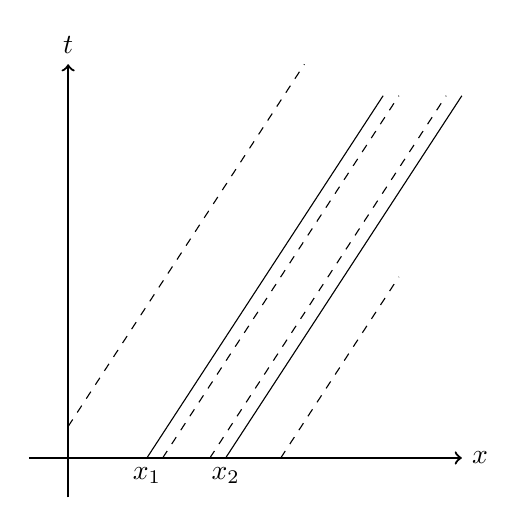
\begin{tikzpicture}
	%axis 
	\draw[->, thick] (-0.5,0)--(5,0) node[right]{$x$};
	\draw[->, thick] (0,-0.5)--(0,5) node[above]{$t$};
	%characteristics
	\draw[dashed] (0,0.4)--(3,5);	
	\draw (1,0) node[below]{$x_1$} --(4,4.6);
	\draw[dashed] (1.2,0)--(4.2,4.6);	
	\draw[dashed] (1.8,0)--(4.8,4.6);	
	\draw (2,0) node[below]{$x_2$} --(5,4.6);	
	\draw[dashed] (2.7,0)--(4.2,2.3);	
\end{tikzpicture}
	\caption{ $X(t,x)$}
\end{figure}

Let us look for $X(t,x)$ such that $\rho(t,X(t,x))$ does not
depend on $t$.

\begin{align*}
	0 = & \frac{\text{d}}{\text{d}t} \rho(t,X(t,x)) \\
	= & \partial_t \rho(t,X(t,x)) +\nabla \rho(t,X(t,x))
	\cdot \partial_t X(t,x)\\
	= & -u(t,X(t,x))\cdot \nabla\rho(t,X(t,x)) +
	\partial_t X(t,x)\nabla\rho(t,X(t,x)) 
\end{align*},
(because $\partial_t \rho(t,x) +u(t,X(t,x))\cdot \nabla\rho(t,x)
=0 \quad \forall x, t$.)

A sufficient condition is $\partial_t X(t,x) = u(t,X(t,x))
\quad \forall t, x$. For $x$ fixed, this is an ODE.

Consider the family of ODE:
\begin{equation}
	\tag{$\mathcal{C}_x$}
	\left\lbrace
	\begin{array}{lclc}
		\partial_{\color{red}{1}} X(t,x) &=& u(t,X(t,x)) \\
	X(0,x) &=& x 
	\end{array}
    \right.
    \label{eq-cxfamily}
\end{equation}

Assumptions: $u$ is continuous with respect to $t$ and $x$
and globally Lipschitz-continuous with respect to $x$:
$$\vert u(t,y) -u(t,x)\vert \leq L\vert y-x\vert \quad
\forall (t,x,y)\in \R\times\R^d\times\R^d$$

Under these assumptions, there exist a unique global situation
to \eqref{eq-cxfamily} for all $x\in\R^d$.

Now, if $\rho$ is constant along $X$,
$$\rho(t,X(t,x)) = \rho(s,X(s,x)) = \rho(0,X(0,x)) = \rho_0(x)$$.

Problem:
If $(t,x)$ is given, how to compute $\rho(t,x)$?

Find $y\in\R^d$ such that $X(t,y) = x$ then
$$\rho(t,x) = \rho(t,X(t,y)) = \rho_0(y)$$.
We have to invent the \definition{characteristic (curve)}
$x\mapsto X(t,x)$ at fixed $t$.
Consider now $X(s,t,x)$ such that
\begin{equation}
	\left\lbrace
	\begin{array}{lclc}
		\partial_1 X(s,t,x) &=& u(s,X(s,t,x)) \\
		X(\underbrace{t}_{\text{real time}},
		\underbrace{t}_{\text{Cauchy datum time}},x) &=& x 
	\end{array}
    \right.
\end{equation}

The solution to this problem satisfies the \definition{semi-group property}
$X(t_3,t_2,X(t_1,x)) = X(t_3,t_1,x)$, consequence of the uniqueness 
of solution.

Consequence: $X(t,0,X(0,t,x)) = X(t,t,x) = x$.

\textbf{Second stage:} Come back to 
\begin{equation}
	\tag{$\mathcal{CNC}$}
	\left\lbrace
	\begin{array}{lclc}
		\partial_t \rho + u\cdot\nabla \rho &=& 0 \\
		\rho(0,\cdot) &=& \rho_0 
	\end{array}
	\label{eq-cnc}
    \right.
\end{equation}.

Saying that $\rho$ is constant along the characteristic is saying that
$$\rho(t,x) = \rho_0(X(0,t,x))$$.
Indeed,  $X(t,0,X(0,t,x)) = x$, thus
\begin{align*}
	\rho(t,X(t,0,X(0,t,x))) & = \rho(t,x)\\
	\rho(0,X(0,0,X(0,t,x))) & = \rho_0(X(0,t,x))
\end{align*}.

We defined characteristic curve along which \textbf{the} solution
$\rho$ has to be a constant. We define $\rho$ as constant along these 
curves $$\rho(t,x) = \rho_0(X(0,t,x))$$.

Is this $\rho(t,x)$ solution to the Cauchy problem?

\begin{proof}
	[First proof]
	Let us prove that 
	$$(\frac{\text{d}}{\text{d}t} + u\cdot\nabla)
	\rho_0(X(0,t,x)) = 0$$.
	
	First, we have:
	$$\frac{\text{d}}{\text{d}t}( \rho_0(X(0,t,x))) 
	= \nabla \rho_0(X(0,t,x))\partial_2X(0,t,x)$$.

	Let us define $g(t,x) = X(t,t,x) = x = X(t,0,X(0,t,x))$.
	Then
	\begin{align*}
		\partial_1 g(t,x) &= 0 \\
		&= \partial_1 X(t,0,X(0,t,x)) + \nabla_3
		 X(t,0,X(0,t,x))\cdot \partial_2 X(0,t,x)\\
		&= u(t, X(t,0,X(0,t,x)))+ \nabla_3
		 X(t,0,X(0,t,x))\cdot \partial_2 X(0,t,x)\\
		&= u(t,x) + \nabla_3
		 X(t,0,X(0,t,x))\cdot \partial_2 X(0,t,x)
	\end{align*}
	
	Thus $\nabla_3 X(t,0,X(0,t,x))\cdot \partial_2 X(0,t,x) = -u(t,x)$.
	
	Then,
	$\nabla(\rho_0(X(0,t,x))) = [\nabla_x\rho_0(X(0,t,x)))]^T
	\cdot \nabla_3X(0,t,x)$

	Compute $\nabla_3X(0,t,x)$:
	$$\nabla_x g(t,x) = I_d = \nabla_x X(t,0,X(0,t,x))\nabla_3X(0,t,x))$$
\begin{rem}
	Thus $\nabla_x X(t,0,X(0,t,x))\equiv A $ is invertible and 
	$A^{-1} = (\nabla_x X(t,0,X(0,t,x)))^{-1} =\nabla_3X(0,t,x)) $.
\end{rem}
	Thus
	\begin{align*}
		& u(t,x)\cdot\nabla_x(\rho_0(X(0,t,x)))\\
		=& u(t,x) \nabla_3X(0,t,x)\nabla_x\rho_0(X(0,t,x))\\
		=& u(t,x) A^{-1} \nabla_x\rho_0(X(0,t,x))
	\end{align*}.
	Finally
	\begin{align*}
		& (\frac{\text{d}}{\text{d}t}+u\cdot\nabla_x)\rho_0(X(0,t,x))\\
		&= \nabla\rho_0(X(0,t,x))\partial_2X(0,t,x)
		+ u \nabla_x(\rho_0(X(0,t,x)))\\
		&= -\nabla\rho_0(X(0,t,x)) A^{-1} u(t,x) 
		+ u [(A^{-1})^T \nabla_x\rho_0(X(0,t,x)))]^T\\
		&= -\nabla\rho_0(X(0,t,x)) A^{-1} u(t,x) 
		+\nabla_x\rho_0(X(0,t,x))) A^{-1} u(t,x) \\
		&= 0
	\end{align*}.
	Conclusion: $(t,x)\mapsto \rho_0(X(0,t,x)) = \rho(t,x)$ is
	a solution to $\partial_t\rho + u\nabla\rho = 0$.
	Furthur more, $\rho(0,x) = \rho_0(X(0,0,x)) = \rho_0(x)$,
	thus $\rho(t,x)$ satisfies the Cauchy datum.
	$\rho(t,x)$ is a solution to the Cauchy problem.
\end{proof}

\begin{proof}
	[Second proof]
	$\rho(t,x) = \rho_0(X(0,t,x))$ is constant along the characteristic.
	$$\rho(t,X(t,t_0,x))=\rho_0(X(0,t,X(t,t_0,x))) = \rho_0(X(0,t_0,x))$$
	which does not depend on $t$.

	Consequence: 
	$\nabla_{t,x}\rho(t,x)$ is perpendicular to the tangent vector
	of $X(t,x)$ who is parallel to $(1,\partial_1 X)^T$.
	Thus, 
	\begin{align*}
		&\partial_t\rho\cdot 1 +\partial_1 X\cdot\nabla_x\rho = 0\\
		\Rightarrow & \partial_t\rho + u\cdot \nabla_x\rho
	\end{align*}.
\end{proof}

Last question: is the solution to \eqref{eq-cnc} unique?

If $ \partial_t\rho + u\cdot \nabla\rho = 0$, $\rho$ is constant 
along the characteristics, thus $\rho(t,x) = \rho(0,X(0,t,x)) = 
\rho_0(X(0,t,x))$, the solution is unique.


\begin{theo}
	Assume $u$ is continuous with respect to $(t,x)$ and
	globally Lipschitz-continuous with respect to $x$.
	The \eqref{eq-cnc} admits a unique global solution given by 
	$\rho(t,x) = \rho_0(X(0,t,x))$ where the curves $X$ are
	solutions to 
\begin{equation}
	\left\lbrace
	\begin{array}{lclc}
		\partial_1 X(s,t,x) &=& u(s,X(x,t,x)) \\
		X(t,t,x) &=& x 
	\end{array}
    \right.
\end{equation}.
\end{theo}

Come back to the continuity equation.
\begin{equation}
	\tag{$\mathcal{CC}$}
	\left\lbrace
	\begin{array}{lclc}
		\partial_t \rho + \nabla\cdot(\rho u) 
		&=& 0 \quad t\in\R\,x\in\R^d \\
		\rho(0,\cdot) &=& \rho_0 
	\end{array}
    \right.
\end{equation}.

\begin{rem}
	For the unconservative equation $\partial_t \rho +u \nabla\rho=0$,
	we see that $D_t\rho = 0$. ($D_t$ is the Lagrangian derivative)
\end{rem}

	Consider $\bar{\rho}(t,x) = \rho(t,X(t,0,x))$ where $\rho$ is a
	solution to \eqref{eq-cc}.
	We have
	\begin{align*}
		\partial_t \bar{\rho}(t,x) 
		&= \partial_t \rho(t,X(t,0,x)) + \partial_1X(t,0,x)
		\nabla\rho(t,X(t,0,x))\\
		&= \partial_t \rho(t,X(t,0,x)) + u(t,X(t,0,x))
		\nabla\rho(t,X(t,0,x))\\
		&= -\rho(t,X(t,0,x))\nabla u(t,X(t,0,x))
	\end{align*}.
	Thus $\partial_t \bar{\rho}(t,x) =
	-\rho(t,X(t,0,x))\nabla u(t,X(t,0,x))$.
	Thus, $\bar{\rho}$ satisfies
	\begin{align*}
		\bar{\rho}(t,x) &= \bar{\rho}(0,x)
		e^{-\int_0^t \nabla u (s,X(s,0,x)) \text{d}s}\\
		\bar{\rho}(0,x) &= \rho(0,X(0,0,x)) = \rho(0,x) = \rho_0(x)\\
		\Rightarrow \bar{\rho}(t,x) &=
		\rho_0(x) e^{-\int_0^t \nabla u (s,X(s,0,x)) \text{d}s}
	\end{align*}.
	We are interested in $\rho$,
	$$\bar{\rho}(t,x) = \rho(t,X(t,0,x)) \Leftrightarrow
	\rho(t,x) = \bar{\rho}(t,X(0,t,x))$$.

	Indeed,
	\begin{align*}
		&\bar{\rho}(t,x) = \rho(t,X(t,0,x)) \quad\forall x\\
		\Leftrightarrow & \bar{\rho}(t,X(0,t,y)) =
		\rho(t,X(t,0,X(0,t,y)))  \quad\forall y\\
		\Leftrightarrow & \bar{\rho}(t,X(0,t,y)) = 
		\rho(t,y) \quad \forall y
	\end{align*}.

	Then
\begin{equation}
	\rho(t,x) = \bar{\rho}(t,X(0,t,x)) 
	= \rho_0(X(0,t,x)) e^{-\int_0^t \nabla u (s,X(s,0,X(0,t,x))) \text{d}s}
	= \rho_0(X(0,t,x)) e^{-\int_0^t \nabla u (s,X(s,t,x)) \text{d}s}
\end{equation}.

\begin{theo}
	Assume $u\in \mathcal{C}^1$ with respect to  $(t,x)$ and
	globally Lipschitz-continuous with respect to $x$.
	Then \eqref{eq-cc} has a unique global solution, given by
	\begin{equation}
	\rho(t,x) 
	= \rho_0(X(0,t,x)) e^{-\int_0^t \nabla u (s,X(s,t,x)) \text{d}s}
	\label{eq-solutionexact}
\end{equation}.

\end{theo}

\begin{rem}
	For \eqref{eq-cnc}, the solution satisfies the maximum principle:
	$$\min_y \rho_0(y) \leq \rho(t,x) \leq \max_y\rho_0(y)$$.
\end{rem}

Indeed, $\rho(t,x) = \rho_0(X(0,t,x))$.

It is the same for \eqref{eq-cc} when $\nabla u =0$.
In the conservative case where $\nabla u \neq 0$, the maximum principle 
is not satisfied.

For the \eqref{eq-cnc}, remember that it models the evolution of a mass fraction
$c=\frac{ \rho_1}{ \rho_1+\rho_2}$. ($c_0\in[0,1]\Rightarrow c(t)\in[0,1]$.)\\
Summary of the mathematical modelling part.\\
Conservative transport equation.
\begin{eqnarray}
\partial_t \rho + \partial_x \rho u = 0, \quad \text{(d = 1)}
\end{eqnarray}
% 2 graphes à faire
PLIC
\begin{eqnarray*}
\rho(t,x) &=& r(t) :\\
0 &=& \partial_t r + \partial_x r u\\
&=& \partial_t r + u \partial_x r + r \partial_x u\\
&=& \partial_t r + r \partial_x u \\
&=& \partial_t r - r\\
\Rightarrow r(t) &=& r(0)e^t = e^t
\end{eqnarray*}
% 2 graphes
For the $(NC)$ equation : 
\begin{equation}
\partial_t \rho + u \partial_x \rho = 0
\end{equation}
with $\rho(t,x) = \rho\left(0,X(0,t,x)\right)$.
% 1 graphe
with $ X(s,t,x) = x e^{-(s-t)}$.
\subsection{Discretisation}
\textbf{\underline{GOAL}} : to compute approximate solutions to : 
\begin{eqnarray}
\partial_t \rho + \nabla.\rho u &=& 0\\
\rho(0,.) &=& \rho^0 
\end{eqnarray} 
and
\begin{eqnarray}
\partial_t \rho + u.\nabla \rho &=& 0\\
\rho(0,.) &=& \rho^0 
\end{eqnarray}
We have explicit formula for these Cauchy problem, but for more complicate problems (cf the following of the course), we will need the technique we will develop here.
We will restrict to the case where $d=1$.

\subsubsection{$\partial_t \rho + u \partial_x \rho = 0$}

General technique : \textbf{finite differences}.
Let $\Delta x>0$ be the space step and $\Delta t>0$ be the time step.
Define 
\begin{eqnarray}
t^n &=& n\Delta t, \quad n \in \N \\
\text{and} \quad x_j &=& j \Delta x , \quad j \in \mathbb{Z} 
\end{eqnarray}
$(\rho^n_j)_{n \in \N, j \in \mathbb{Z}}$ is intended to approximate $\left(\rho(t^n,x_j)\right)_{n \in \N, j \in \mathbb{Z}}$ where $\rho$ is the solution to : 
\begin{eqnarray}
\partial_t \rho + u \partial_x \rho &=& 0 \\
\rho(0,.) &=& \rho^0
\end{eqnarray}
A finite difference algorithm to define $(\rho^n_j)$ is (assuming $u = cst$) :
\begin{eqnarray}
\frac{\rho^{n+1}_j - \rho^n_j}{\Delta t} + u \frac{\rho^{n}_{j+1} - \rho^n_{j-1}}{2\Delta x} &=& 0\\
\text{or} \quad \frac{\rho^{n+1}_j - \rho^n_j}{\Delta t} + u \frac{\rho^{n}_{j} - \rho^n_{j-1}}{\Delta x} &=& 0\\
\text{or} \quad \frac{\rho^{n+1}_j - \rho^n_j}{\Delta t} + u \frac{\rho^{n}_{j+1} - \rho^n_{j}}{\Delta x} &=& 0\\
\text{or} \quad \frac{\rho^{n+1}_j - \rho^n_j}{\Delta t} + u \frac{\rho^{n+1}_{j+1} - \rho^{n+1}_{j-1}}{2\Delta x} &=& 0
\end{eqnarray} 
Here we restrict to : \textbf{explicit} schemes : the discrete time derivative only involves the time index $n$ (not $n+1$).
It is natural to initialize the time sequence with : 
\begin{eqnarray}
\rho^{n+1}_j &=& \rho^n_j - u\frac{\Delta t}{\Delta x}\left(\rho^n_j - \rho^n_{j-1}\right) \\
\rho^0_j &=& \rho^0(x_0)
\end{eqnarray}
\theorem{Lemma} : This scheme is consistant at first order.
\definition{The consistency error} : 
\begin{eqnarray}
\varepsilon^n_j(\rho) = \frac{\rho(t^{n+1} ,x_{j}) - \rho(t^{n} ,x_{j})}{\Delta t} + u \frac{\rho(t^{n} ,x_{j}) - \rho(t^{n} ,x_{j-1})}{\Delta x}
\end{eqnarray}
Then, if the solution $\rho$ is smooth enough ($\rho \in \mathcal{C}^2_U (\R_{+} \times \R)$ : the first and second derivative of $\rho$ are uniformly bounded on $\R_{+} \times \R$), there exists a constant $C$ s.t. 
\begin{equation}
\vert \varepsilon^n_j \vert \le C(\Delta t + \Delta x),\qquad \forall n \in \N,\quad  j \in \mathbb{Z}
\end{equation}
\textbf{PROOF}.
\begin{eqnarray*}
\frac{\rho(t^{n+1} ,x_{j}) - \rho(t^{n} , x_{j})}{\Delta t} &=& \partial_t  \rho(t^n, x_j) + \underbrace{\mathcal{O}(\Delta t)}_{\text{unif. bounded w.r.t. } j\text{ and }n} \\
\frac{\rho(t^{n} ,x_{j}) - \rho(t^{n} ,x_{j-1})}{\Delta x} &=& \partial_x \rho(t^n, x_j) + \mathcal{O}(\Delta x) \\
\Rightarrow \frac{\rho(t^{n+1} ,x_{j}) - \rho(t^{n} ,x_{j-1})}{\Delta t} 
+u\frac{\rho(t^{n} ,x_{j}) - \rho(t^{n} ,x_{j-1})}{\Delta x}   
&=& \partial_t \rho(t^n,x_j) + u \partial_x \rho(t^n,x_j) + \mathcal{O}(\Delta t + \Delta x) \\
&=& 0 + \mathcal{O}(\Delta t + \Delta x)\quad  (\text{because} \partial_t \rho + u \partial_x \rho).
\end{eqnarray*}
Thus, 
\begin{eqnarray*}
\vert \varepsilon^n_j \vert = \mathcal{O}(\Delta t + \Delta x)
\le  C (\Delta t + \Delta x). 
\end{eqnarray*}
\theorem{Theorem} : Assume $\rho \in C^2_U(\R_{+} \times \R)$
($\rho^0 \in C^2_U(\R)$ is sufficient, because : $\rho(t,x) =\rho^0(x-ut)$.)
Assume $u \ge 0$. \\
Assume $u\Delta t \le \Delta x$.
Then, the scheme : 
\begin{eqnarray}
\frac{\rho^{n+1}_{j} - \rho^{n}_{j}}{\Delta t} + u \frac{\rho^{n}_{j} - \rho^{n}_{j-1}}{\Delta x} &=& 0 \\
\rho^0_j &=& \rho^0(x_j)
\end{eqnarray}
is convergent at the first order :
\begin{equation}
\exists C / \vert \underbrace{\rho^n_j - \rho(t^n,x_j)}_{e_j^n}\vert \le C t^n (\Delta t + \Delta x) \forall n, \forall j
\end{equation}
\textbf{PROOF}. Let's define :
\begin{eqnarray}
e_j^n &=& \rho^n_j - \rho(t^n,x_j) \\
\Rightarrow e_j^{n+1} &=& \rho^{n+1}_j - \rho(t^{n+1},x_j) \\
&=& \rho^n_j - u \frac{\Delta t}{\Delta x}(\rho^n_j - \rho^n_{j-1}) - \rho(t^{n+1},x_j)
\end{eqnarray}
Recall that : 
\begin{eqnarray}
\varepsilon_j^n = \frac{\rho(t^{n+1},x_j)-\rho(t^n,x_j)}{\Delta t} + u \frac{\rho(t^{n},x_j)-\rho(t^n,x_{j-1})}{\Delta x} 
\end{eqnarray}
Thus : 
\begin{eqnarray}
e_j^{n+1} &=& \rho_j^n - u\frac{\Delta t}{\Delta x}\left(\rho_j^n - \rho^n_{j-1}\right) - \left(\rho(t^{n},x_j) -  u\frac{\Delta t}{\Delta x} (\rho(t^{n},x_j)-\rho(t^n,x_{j-1}) + \Delta t \epsilon^n_j \right). \\
&=& e^n_j - u\frac{\Delta t}{\Delta x} (e^n_j - e^n_{j-1}) - \Delta t \varepsilon^n_j
\end{eqnarray}
$(e^n_j)$ satisfies the same scheme as $(\rho_j^n)$ with a source term $\Delta t \varepsilon_j^n$.
So : 
\begin{equation}
e_j^{n+1} = e_j^n \left(1 - u\frac{\Delta t}{\Delta x}\right) + e^n_{j-1} u\frac{\Delta t}{\Delta x} + \Delta t \varepsilon_j^n  
\end{equation}
Thus :
\begin{equation}
\vert e^{n+1}_j \vert \le \vert e^n_j \vert . \vert 1 - u\frac{\Delta t}{\Delta x} \vert  + \vert e^n_{j-1} \vert . \vert u\frac{\Delta t}{\Delta x} \vert + \Delta t \vert \varepsilon^n_j \vert
\end{equation}
Under the assumptions $u \ge 0$ and $u\Delta t \le \Delta x$, we have :
\begin{equation}
\vert u\frac{\Delta t}{\Delta x} \vert = u\frac{\Delta t}{\Delta x} 
\end{equation}
and
\begin{equation}
\vert 1-u\frac{\Delta t}{\Delta x} \vert= 1 - u\frac{\Delta t}{\Delta x}
\end{equation}
\begin{eqnarray}
\vert e^{n+1}_j \vert & \le & \vert e^{n}_j \vert \left(1 - u\frac{\Delta t}{\Delta x}\right) + \vert e^n_{j-1} \vert u\frac{\Delta t}{\Delta x} + \Delta t \vert \varepsilon_j^n \vert \\
&\le & \underbrace{\Vert e^n \Vert_\infty}_{\sup_{j \in \mathbb{Z}}\vert e^n_j \vert} \left(1 - u\frac{\Delta t}{\Delta x} + u\frac{\Delta t}{\Delta x} \right) + \Delta t \vert \varepsilon^n_j \vert \\
&\le & \Vert e^n \Vert_\infty + \Delta t \vert \varepsilon_j^n \vert \\
&\le & \Vert e^n \Vert_\infty + \Delta t \underbrace{\Vert \varepsilon^n \Vert_\infty}_{\sup_{j \in \mathbb{Z}}\vert \varepsilon^n_j \vert} \\
\Rightarrow  \Vert e^{n+1} \Vert_\infty &\le & \Vert e^n \Vert_\infty + \Delta t \Vert \varepsilon^n \Vert_\infty \\
& \le &  \underbrace{\Vert e^0 \Vert_\infty}_{=0} + \Delta t \sum_{k=0}^{n} \Vert \varepsilon^k \Vert_\infty \quad \text{via Discrete Gronwall Lemma} \\
\Rightarrow \Vert e^{n} \Vert_\infty & \le & \Delta t \sum_{k=0}^{n-1} \Vert \varepsilon^k \Vert_\infty
\end{eqnarray}
Thanks to the \textbf{consistency} Lemma : 
\begin{eqnarray}
\Vert e^n \Vert_\infty & \le & C \Delta t \sum_{k=0}^{n-1} (\Delta t + \Delta x) \\
&=& C\Delta t n (\Delta t + \Delta x) \\
&=& C t^n (\Delta t + \Delta x)
\end{eqnarray}
\underline{\textbf{Remarks}}. 
\begin{itemize}
\item $u \ge 0$ is very important.
Without this assumption, we are not able to prove the stability .
\item $u\frac{\Delta t}{\Delta x} \le 1 $ also.
This condition is called the Courant-Friedrichs-Lewy (CFL) (stability) condition. This expresses the fact that the \textbf{\underline{exact}} solution does not cross more than one space cell in a time step.
\item The estimate is not uniform in time, we are not able to bound $\sup_n \Vert e^n \Vert_\infty $ but it is a good estimate locally in time (for a fixed time).
\end{itemize}
We are working on the upwind schemes.\\
\definition{Upwind} : the information comes from the "correct" side :
\begin{itemize}
\item from the left to the right if $u \ge 0$ (not convergent), (RW) scheme ;
\item from the right to the left if $u \le 0$ (convergent), (LW) scheme.
\end{itemize}
For $u \ge 0$, the scheme 
\begin{equation}
\frac{\rho^{n+1}_j - \rho^n_j}{\Delta t} + u \frac{\rho^{n}_{j} - \rho^n_{j-1}}{\Delta x} = 0,\qquad u \ge 0 \quad (RW)
\end{equation}
does not satisfy the same stability property : 
\begin{equation}
\rho_j^{n+1} = \rho^n_j (1 + u\frac{\Delta t}{\Delta x}) + \rho^n_{j+1}(-u\frac{\Delta t}{\Delta x})
\end{equation}
\textbf{This is not a convex combination ! }
It is possible to prove that the scheme is not convergent. \\
The scheme is \textbf{not convergent}. \\
For $u \le 0$, the scheme
\begin{equation}
\frac{\rho^{n+1}_j - \rho^n_j}{\Delta t} + u \frac{\rho^{n}_{j+1} - \rho^n_j}{\Delta x} = 0, \qquad u \le 0 \quad (LW)
\end{equation}
is convergent.\\
The centered scheme is : 
\begin{eqnarray}
\frac{\rho^{n+1}_j - \rho^n_j}{\Delta t} + u \frac{\rho^{n}_{j+1} - \rho^n_{j-1}}{2\Delta x} &=& 0, \quad \forall n,j \\
\rho^0_j &=& \rho^0(x_j)
\end{eqnarray}
\theorem{Lemma} : if $\rho \in C^3_U(\R_{+} \times \R)$,
\begin{equation}
\exists C,\quad \vert \varepsilon_j^n \vert \le C (\Delta t + \Delta x^2)
\end{equation}  
with 
\begin{equation}
\varepsilon^n_j = \frac{\rho(t^{n+1},x_j)-\rho(t^n,x_j)}{\Delta t} + u\frac{\rho(t^{n},x_{j+1})-\rho(t^n,x_{j-1})}{2\Delta x}
\end{equation}
\begin{proof}
	See \ref{ans1}.
\end{proof}

\underline{\textbf{Study the stability}}. \\
\begin{equation}
\rho^{n+1}_j = \rho_j^n + \rho^n_{j-1}\left(u \frac{\Delta t}{2\Delta x} \right) + \rho^n_{j+1} \left(-u \frac{\Delta t}{2\Delta x} \right)
\end{equation}
This is not a convex combination of the $\rho^n_k$ !\\
The scheme is not stable in the norm $\Vert . \Vert_\infty$ in the sense that we do not have : $\Vert \rho^{n+1} \Vert_\infty \le \Vert \rho^{n} \Vert_\infty$. \\
Actually, an inequality as :
\begin{equation}
\Vert \rho^{n+1} \Vert_\infty \le \Vert \rho^{n} \Vert_\infty (1 + C\Delta t) \qquad \text{(we assume this is true !)}  
\end{equation}
would be enough.\\
Indeed, it would ensure :
\begin{eqnarray}
\Vert \rho^n \Vert_\infty & \le & \Vert \rho^0 \Vert_\infty (1 + C\Delta t)^n \\
& \le & \Vert \rho^0 \Vert_\infty e^{Cn\Delta t} \\
&=& \Vert \rho^0 \Vert e^{Ct^n}
\end{eqnarray}
We can prove that \footnote{See \ref{ans3}} :
\begin{equation}
e_j^{n+1} = e_j^n + u\frac{\Delta t }{2 \Delta x}e_{j-1}^n - u\frac{\Delta t }{2 \Delta x}e_{j+1}^n - \Delta t \varepsilon^n_j 
\end{equation}

Consequence of this is concerning the error analysis :
\begin{equation}
\Vert e^{n+1}\Vert_\infty \le \Vert e^{n}\Vert_\infty (1 + C\Delta t) + \Delta t \Vert \varepsilon^n \Vert_\infty  
\end{equation}
Thanks to a discrete Gronwall Lemma 
\footnote{Proof in exercice, see \ref{ans4}},
\begin{equation}
\Vert e^n \Vert_\infty \le \Vert e^0 \Vert_\infty e^{Ct^n} + \sum_{k=0}^{n-1} \Vert \varepsilon^k \Vert_\infty e^{C(t^n - t^k)}
\end{equation}


and finally :
\begin{equation}
\Vert e^n \Vert_\infty \le e^{Ct^n}n \Delta t \sup_{n} \Vert \epsilon^n  \Vert_\infty
\end{equation}
This \textbf{would be} a convergence estimate.\\
With the present scheme, it is possibleto prove that :
\begin{equation}
\Vert \rho^{n+1} \Vert_2 \le \Vert \rho^n \Vert_2 (1 + C\Delta t)
\end{equation}
\textbf{PROOF}. \\
Let us prove this estimation : 
\begin{equation}
\Vert \rho^n \Vert_2 = \left(\sum_j (\rho_j^n)^2 \right)^{1/2}
\end{equation}
We have :
\begin{eqnarray}
\left(\rho_j^{n+1}\right)^2 &=& \left(\rho^n_j + u\frac{\Delta t }{2 \Delta x}\rho_{j-1}^n - u\frac{\Delta t }{2 \Delta x}\rho_{j+1}^n \right)^2 \\
&=& \left(\rho^n_j + \frac{\nu}{2}\rho_{j-1}^n - \frac{\nu}{2}\rho_{j+1}^n \right)^2, \quad \text{(with } \nu = u\frac{\Delta t }{2 \Delta x} \text{ the Courant number)} \\
&=& {\rho^n_j}^2 + \frac{\nu^2}{4}{\rho_{j-1}^n}^2 - \frac{\nu^2}{4}{\rho_{j+1}^n}^2 + \nu \rho^n_j \rho_{j-1}^n - \nu \rho_{j}^n \rho_{j+1}^n - \frac{\nu^2}{2}\rho_{j-1}^n \rho_{j+1}^n \\
& \le & {\rho_j^n}^2 + \frac{\nu^2}{4}({\rho_{j-1}^n}^2 {\rho_{j+1}^n}^2) + \frac{\nu^2}{4} ({\rho_{j-1}^n}^2 + {\rho_{j+1}^n}^2) + \nu \rho_{j}^n(\rho_{j-1}^n - \rho_{j+1}^n)
\end{eqnarray}
(because $ab < \frac{a^2+b^2}{2}$). \\
Then :
\begin{eqnarray}
\sum_j \left(\rho_j^{n+1}\right)^2 & \le & \sum_j \left(\rho_j^{n}\right)^2 (1 + \nu^4) + 0 \\
\sum_j \left(\rho_j^{n+1}\right)^2 & \le & \sum_j \left(\rho_j^{n}\right)^2 \underbrace{(1 + u^2 \frac{\Delta t^2}{\Delta x^2})}_{1+C\Delta t}
\end{eqnarray}
If $u^2 \frac{\Delta t^2}{\Delta x^2} = C\Delta t$, then : 
$$ u^2 \Delta t = C \Delta x^2 \Rightarrow \Delta t = C \frac{\Delta x^2}{u^2}.$$
\textbf{RESULTS}. \\
If $\Delta t = C \frac{\Delta x^2}{u^2}$, one has :
\begin{equation}
\Vert \rho^{n+1} \Vert_2 \le \Vert \rho^n \Vert_2 (1+C\Delta t)
\end{equation}
and the scheme is convergent in the norm $\Vert . \Vert_2$.
Note that this is false for the $\underbrace{\textbf{\underline{downwind}}}_{(\textit{load})}$ scheme.\\
\underline{\textbf{Remark}} : this scheme is not to be used because very costly due to $\Delta t \sim D\Delta x$.
Other technique to prove the stability in $\ell^2$ : by \textbf{Fourier Transform}.\\
Assume that $(\rho^n)_j \in \ell^2$.
Let us define : 
\begin{eqnarray}
\rho^n \Delta(x) &=& \sum_{j \in \mathbb{Z}} \rho^n_j \mathrm{1}_{c_j}(x) \\
\text{with}\quad c_j &=& \left[x_j - \frac{\Delta x}{2}; x_j + \frac{\Delta x}{2}\right[
\end{eqnarray}
We have $\rho^n \Delta \ in L^2$ and $\Vert \rho^n\Delta \Vert_{L^2} = \sqrt{\Delta x} \Vert \rho ^n \Vert_{\ell^2}$. \\
For any $f \in L^2(\R)$, define :
\begin{equation}
\hat{f}(\xi) = \int_{\R}f(x)e^{-ix\xi} dx
\end{equation}
Thanks to the Perseval identity, $\Vert \hat{f} \Vert_{L^2} =  \Vert f \Vert_{L^2}$.\\
Furthermore, $\hat{f(.+\tau)}(\xi) = \hat{f}(\xi)e^{i\tau\xi}$.
Consider the scheme :
\begin{equation}
\rho_j^{n+1} = \rho^n_j + u\frac{\Delta t}{2\Delta x}\rho^n_{j-1} - u\frac{\Delta t}{2\Delta x}\rho^n_{j+1} 
\end{equation}
We have :
\begin{eqnarray}
\rho^{n+1}\Delta &=& \rho^{n}\Delta + u\frac{\Delta t}{2\Delta x}\rho^n\Delta(.-\Delta x) - u\frac{\Delta t}{2\Delta x}\rho^n\Delta(.+\Delta x)\\
\Rightarrow \Vert \rho^{n+1}\Delta \Vert_{\ell^2} &=& \frac{1}{\sqrt{\Delta x}}\Vert \rho^{n+1}\Delta\Vert_{L^2} 
\end{eqnarray}
\begin{eqnarray}
\hat{\rho^{n+1}}\Delta(\xi) &=& \hat{\rho^{n}}\Delta(\xi) + \frac{\nu}{2}\hat{\rho^{n}}\Delta(\xi)e^{-i\xi\Delta x} - \frac{\nu}{2}\hat{\rho^{n}}\Delta(\xi)e^{i\xi\Delta x}\\
&=& \hat{\rho^n}\Delta(\xi)\left(1 - \frac{\nu}{2}(e^{i\xi\Delta x}-e^{-i\xi\Delta x})\right) \\
&=& \hat{\rho^n}\Delta(\xi)\left(1 - i\nu \sin(\xi\Delta x)\right)
\end{eqnarray} 
Thus, 
\begin{eqnarray}
\Vert \rho^{n+1} \Vert_{\ell^2} &\le & \frac{1}{\sqrt{\Delta x}}\Vert \hat{\rho^{n}}\Delta\Vert_{L^2} \sup_{\xi} \vert 1-i\nu \sin(\xi\Delta x)\vert \\
&=& \Vert \rho^n \Vert_{\ell^2} \sup_{\xi} \vert 1-i\nu \sin(\xi\Delta x)\vert \\
&=& \Vert \rho^n \Vert_{\ell^2} \sup_{\xi} \left(1+\nu^2 \sin(\xi\Delta x)\right)^{\frac{1}{2}}
\end{eqnarray}
We recover the condition : $\Delta t = D\Delta x^2$ in order the amplification factor $1 - i\nu \sin(\xi\Delta x)$ to be uniformly bounded (w.r.t. $\xi$) by $(1+C\Delta t)$.\\
\textbf{Exercise}. \\
The Lax-Wendroff scheme is :
\begin{equation}
\rho_j^{n+1} = \rho_j^{n} - \frac{\nu}{2}\left(\rho^n_{j+1} - \rho^n_{j-1} \right) + \frac{\nu^2}{2}\left(\rho^n_{j+1} - 2\rho^n_{j} + \rho^n_{j-1}\right)
\end{equation}
Prove that this scheme is $2^{nd}$ order (in $\Delta t$ and $\Delta x$) consistent.
Prove that the scheme is $\ell^2$-stable $\left(\Vert \rho^{n+1}\Vert_{\ell^2} \le \Vert \rho^{n}\Vert_{\ell^2}\right)$ \quad (and convergent) under the CFL condition $\nu \le 1$.

\begin{proof}
See \ref{ans2}.	
\end{proof}


%20181010

\begin{recall}
	We have convergence of the upwind scheme for 
	$\partial_t\rho + u\partial_x\rho = 0$ under the
	CFL condition $\frac{u\Delta t}{ \Delta x} \le 1$.
	We have convergence of the centered scheme if
	$\Delta t \sim \Delta x^2$. However, the centered scheme
	is not interesting.
\end{recall}

\underline{Q: In the case where $u$ is not constant?}

There is a natural discretisation:
\begin{equation}
	\frac{ \rho^{n+1}_j - \rho^n_j}{ \Delta t}
	+ u^n_j \frac{ \rho^n_{j+\frac{1}{2}} 
	- \rho^n_{j-\frac{1}{2}}}{ \Delta x} = 0 
\end{equation}
with a formula to compute $\rho^n_{j+\frac{1}{2}}$ as a 
function of $\rho^n_k$.

If for all $j$ and $n$, $u^n_j\ge 0$, then 
$\rho^n_{j+\frac{1}{2}} = \rho^n_j$ is the upwind scheme and
\begin{equation}
	\rho^{n+1}_j = \rho^n_j(1-u^n_j \frac{ \Delta t}{ \Delta x})
	+ u^n_j \frac{ \Delta t}{ \Delta x} \rho^n_{j-1}
\end{equation}.

If for all $j$ and $n$, $u^n_j\frac{ \Delta t}{ \Delta x} \le 1$,
we recover the maximum priciple:
\begin{equation}
	\vert \rho^{n+1}_j \vert \le \sup_k \vert\rho^n_k\vert
\end{equation}.

And the error of the scheme $e^n_j = \rho^n_j - \rho(t^n,x_j)$
satisfies
\begin{equation}
	e^{n+1}_j = e^n_j(1-u^n_j \frac{ \Delta t}{ \Delta x})
	+ e^n_{j-1} u^n_j \frac{ \Delta t}{ \Delta x} 
	- \Delta t \varepsilon^n_j
\end{equation}.

\begin{exercise}
	\begin{itemize}
\item Prove that 
	$\vert\varepsilon^n_j\vert\le C(\Delta t + \Delta x)$ if
	$\rho$ is smooth.
\item Prove the convergence of the scheme under the CFL condition.
	\end{itemize}
\end{exercise}

\begin{proof}
	See \ref{sec-ans-1009-1}.
\end{proof}

\underline{Q: And when $u$ changes sign?}

Naively, we can define:
\begin{equation}
	\rho^n_{j+\frac{1}{2}} = \left\lbrace
	\begin{array}{ll}
		\rho^n_j & \text{ if } u^n_j \ge 0\\
		\rho^n_{j+1} & \text{ if not. }
	\end{array}\right.
\end{equation}
and
\begin{equation}
	\rho^n_{j-\frac{1}{2}} = \left\lbrace
	\begin{array}{ll}
		\rho^n_{j-1} & \text{ if } u^n_j \ge 0\\
		\rho^n_j & \text{ if not }
	\end{array}\right.
\end{equation}.
But then 
\begin{align*}
	u^n_j\ge 0 &\Rightarrow \rho^n_{j+\frac{1}{2}} 
	= \rho^n_j  \text{ (Left winded)} \\
	u^n_{j+1}< 0 &\Rightarrow \rho^n_{j+\frac{1}{2}} 
	= \rho^n_{j+1}  \text{ (Right winded)}  \\
\end{align*}
the results are not compatibles.

Consider another idea, we write a scheme in the form
\begin{equation}
	\rho^{n+1}_j = \rho^n_j
	-u^n_{j+\frac{1}{2}} \frac{ \Delta t}{ \Delta x}
	(\rho^n_{j+\frac{1}{2}} - \rho^n_j)
	-u^n_{j-\frac{1}{2}} \frac{ \Delta t}{ \Delta x}
	( \rho^n_j - \rho^n_{j-\frac{1}{2}})
\end{equation}
with $u^n_{j+\frac{1}{2}} = u(t^n,(j+\frac{1}{2})\Delta x)$.
And we can upwind the interface value.
\begin{equation}
	\rho^n_{j+\frac{1}{2}} = \left\lbrace
	\begin{array}{ll}
		\rho^n_j & \text{ if } u^n_{j+\frac{1}{2}} \ge 0\\
		\rho^n_{j+1} & \text{ if not }
	\end{array}\right.
\end{equation}.
This leads to the scheme
\begin{align*}
	\rho^{n+1}_j & = \rho^n_j
	-(u^n_{j+\frac{1}{2}})^+ \frac{\Delta t}{\Delta x}\cdot 0
	+(u^n_{j+\frac{1}{2}})^- \frac{\Delta t}{\Delta x}
	(\rho^n_{j+1} - \rho^n_j)
	-(u^n_{j-\frac{1}{2}})^+ \frac{\Delta t}{\Delta x}
	(\rho^n_j - \rho^n_{j-1})
	+(u^n_{j-\frac{1}{2}})^+ \frac{\Delta t}{\Delta x}\cdot 0
	\\ &=
	\rho^n_j\left(1-(u^n_{j+\frac{1}{2}})^-\frac{\Delta t}{\Delta x}
	-(u^n_{j-\frac{1}{2}})^+ \frac{\Delta t}{\Delta x}\right)
	+(u^n_{j+\frac{1}{2}})^- \frac{\Delta t}{\Delta x}\rho^n_{j+1}
	+(u^n_{j-\frac{1}{2}})^+ \frac{\Delta t}{\Delta x}\rho^n_{j-1}
\end{align*}.
Assume that $\frac{\Delta t}{\Delta x}\left[(u^n_{j+\frac{1}{2}})^- 
+ (u^n_{j-\frac{1}{2}})^+ \right]\le 1$
\footnote{Consider $(u^n_{j+\frac{1}{2}})^- + (u^n_{j-\frac{1}{2}})^+ $ as a numerical approximation for $\vert u\vert$. This is coherent to
the CFL condition that we've seen before.},
then $\rho^{n+1}_j$ is a convexe combination of
$\rho^n_{j+1}$, $\rho^n_j$ and $\rho^n_{j-1}$,
thus $\vert\rho^{n+1}_j\vert\le\sup_k\vert\rho^n_j\vert$.

\begin{exercise}
	\begin{itemize}
\item Prove that the scheme is consistent.
\item Prove that it is convergent under the CFL condition.
	\end{itemize}
\end{exercise}

\begin{proof}
	See \ref{sec-ans-1009-2}.
\end{proof}

For the conservative equation: $\partial_t\rho+\partial_x\rho u =0$.
(With $u$ non constant, smooth and given).
Natuarally, we have
\begin{equation}
	\rho^{n+1}_j = \rho^n_j
	-\frac{ \Delta t}{ \Delta x}
	(\rho^n_{j+\frac{1}{2}}u^n_{j+\frac{1}{2}} 
	- \rho^n_{j-\frac{1}{2}}u^n_{j-\frac{1}{2}} )
\end{equation}
with $u^n_{j+\frac{1}{2}} = u(t^n,(j+\frac{1}{2})\Delta x)$.
And we can define the upwind interface values:
\begin{equation}
	\rho^n_{j+\frac{1}{2}} = \left\lbrace
	\begin{array}{ll}
		\rho^n_j & \text{ if } u^n_{j+\frac{1}{2}} \ge 0\\
		\rho^n_{j+1} & \text{ if not }
	\end{array}\right.
\end{equation}.

\underline{Q: Do we have the maximum principle? NO!}
Because the exact solution to $\partial_t\rho +\partial_x\rho u=0$
does not satisfy the maximum principle. 
($\partial_t\rho +u\partial_x\rho= \rho\partial_x u$.)
But,
\begin{equation}
	\rho^{n+1}_j = \rho^n_j
	-\frac{\Delta t}{\Delta x} u^n_{j+\frac{1}{2}}
	(\rho^n_{j+\frac{1}{2}} - \rho^n_j)
	-\frac{\Delta t}{\Delta x} u^n_{j-\frac{1}{2}} 
	( \rho^n_j - \rho^n_{j-\frac{1}{2}})
	-\frac{ \Delta t}{ \Delta x}\rho^n_j
	( u^n_{j+\frac{1}{2}}- u^n_{j-\frac{1}{2}})
\end{equation}.
Thus, under the CFL condition ( $\frac{\Delta t}{\Delta x}
\left[(u^n_{j+\frac{1}{2}})^- + (u^n_{j-\frac{1}{2}})^+ \right]\le 1$),
we have:
\begin{align*}
	\vert\rho^{n+1}_j\vert &\le \sup_k\vert\rho^n_k\vert
	+\frac{\Delta t}{\Delta x}\vert\rho^n_j\vert\cdot
	\vert u^n_{j+\frac{1}{2}} - u^n_{j-\frac{1}{2}}\vert \\
	&\le \sup_k\vert\rho^n_k\vert
	+\Delta t\vert\rho^n_j\vert\cdot\Vert\partial_x u\Vert_\infty\\
	&\le \sup_k\vert\rho^n_k\vert
	(1+\Delta t\Vert\partial_x u\Vert_\infty)\\
	\Rightarrow\vert\rho^n_j\vert &\le\sup_k\vert\rho^0_k\vert
	e^{n\Delta t\Vert\partial_x u\Vert_\infty}\quad\forall j
\end{align*}

\begin{rem}
	Compare this to the expression of the exact solution.
\end{rem}

The error satisfies 
\begin{equation}
	\vert e^{n+1}_j\vert \le  \sup_k\vert e^n_k\vert
	(1+\Delta t\Vert\partial_x u\Vert_\infty)
	+ \Delta t \vert \varepsilon^n_j\vert 
\end{equation}
with
\begin{align*}
	\varepsilon^n_j = 
	\frac{\rho(t^{n+1},x_j)-\rho(t^n,x_j)}{ \Delta t}
	& +\frac{[u(t^n,x_{j+\frac{1}{2}})]^+\rho(t^n,x_j)
	-[u(t^n,x_{j+\frac{1}{2}})]^-\rho(t^n,x_{j+1})}{ \Delta x}\\
	& +\frac{[u(t^n,x_{j-\frac{1}{2}})]^+\rho(t^n,x_{j-1})
	-[u(t^n,x_{j-\frac{1}{2}})]^-\rho(t^n,x_j)}{ \Delta x}
\end{align*}
(where $x_{j+\frac{1}{2}}=(j+\frac{1}{2})\Delta x$).

\begin{exercise}
	Prove that there exists $C$ such that
	$\vert\varepsilon^n_j\vert \le C(\Delta t+\Delta x)$.
\end{exercise}

Thus 
\begin{equation}
	\vert e^{n+1}_j\vert \le  \sup_k\vert e^n_k\vert
	(1+\Delta t\Vert\partial_x u\Vert_\infty)
	+ \Delta t  C(\Delta t+\Delta x)
\end{equation}.
Thanks to a discrete Gronwall Lemma,
\begin{align*}
	\exists C \quad	\vert e^n_j\vert 
	&\le\sup_k\vert e^0_k\vert
	e^{n\Delta t\Vert\partial_x u\Vert_\infty}
	+ \sum^{n-1}_{l=0} \Delta t  C(\Delta t+\Delta x)
	e^{(n-l)\Delta t\Vert\partial_x u\Vert_\infty}\\
	&\le n \Delta t  C(\Delta t+\Delta x)
	e^{n\Delta t\Vert\partial_x u\Vert_\infty}
\end{align*}.
The scheme is first order convergent.

\begin{rem}
	The numerical analysis of transport equation is more difficult
	than their analysis. This is due to the fact that there
	is no (simple) formula to express $\rho^n_j$ as a function
	of the $\rho^0_k$. 
	Precisely, there is no $k$ such that $\rho^n_j = \rho^0_k$,
	although for $\partial_t\rho+u\partial =0$, we have
	$\rho(t,x) = \rho(0,X(0,t,x)) = \rho(0,t)$, except when
	$u$ is constant and $u \frac{ \Delta t}{ \Delta x}=1$
	(for the upwind scheme).
\end{rem}

Indeed, if $u>0$,
\begin{equation}
	\rho^{n+1}_j = \rho^n_j - u\frac{ \Delta t}{ \Delta x}
	(\rho^n_j - \rho^n_{j-1})
	= \rho^n_j - (\rho^n_j - \rho^n_{j-1})
	= \rho^n_{j-1}
\end{equation}
and $ \rho^n_j = \rho^0_{j-n})$.
In this case, the scheme is exact. ($\rho(t^n,x_j)=\rho(0,x_{j-n})$)

Transport equations in bounded domain are very complicate problems
(cf. practical session). In dimension $1$, consider
\begin{equation}
	\left\lbrace
	\begin{array}{rl}
		\partial_t\rho +u\partial_x\rho =& 0\\
		\rho(0,x) =& \rho_0(x)
	\end{array}
	\right. t>0\,x\in [0,1]
\end{equation}.
It is natural to impose the value of $\rho$ on the inflow boundary
$x=0$ if $u>0$; $x=1$ if $u<0$.

Indeed, consider that $u>0$, then $\rho(t,x=1)=\rho(0,1-ut)$.
For $t$ sufficiently small, $1-ut\in (0,1)$, thus we cannot ask
$\rho(t,x=1)$ to be equal to a boundary datum.
Conversely, $\rho(t,x=0)=\rho(0,\underbrace{0-ut}_{\not\in (0,1)})$.
Thus in this case ($u>0$), the problem
\begin{equation}
	\left\lbrace
	\begin{array}{rll}
		\partial_t\rho +u\partial_x\rho =& 0
		&  t>0\,x\in [0,1]\\
		\rho(0,x) =& \rho_0(x)
		&  x\in [0,1]\\
		\rho(t,0) =& \rho_0(t) 
		& \text{ given}
	\end{array}
	\right.
\end{equation}
is well posed.
In dimension $d>1$, the condition has to be imposed on 
$x\in\partial\Omega$ where $u\cdot \mathbf{n} >0$.



\subsection{Generalization of transport equation: 
hyperbolic Systems}

\begin{definition}
	The PDE system $\partial_t u + A\partial_x u =0\in\R^n$,
	$t\in\R^+$, $x\in\R$, where $u(t,x)\in\R^n$ and $A\in
	\mathcal{M}(\R)$ is said \definition{hyperbolic} if
	$A$ is $\R$-diagonalizable; \definition{strictly hyperbolic} 
	if $A$ has $n$ distinct real eigenvalues.
\end{definition}

Consider
\begin{equation}
	\left\lbrace
	\begin{array}{rll}
		\partial_t u+A\partial_x u =& 0 & t>0,\,x\in\R\\
		u(0,\cdot)& = u^0&
	\end{array}\right.
\end{equation}
and assume the system is hyperbolic.
$A=PDP^{-1}$ where $D$ is a real diagonal matrix. We have
\begin{align*}
	&P^{-1}(\partial_t u ) + P^{-1} A\partial_x u =0\\
	&\partial_t(P^{-1}u) + P^{-1}AP\partial_x(P^{-1}u) = 0\\
	&\partial_t(P^{-1}u) + D\partial_x(P^{-1}u) = 0\\
	\forall k\quad 
	&\partial_t(P^{-1}u)_k + D_{kk}\partial_x(P^{-1}u)_k = 0\\
	\Rightarrow & (P^{-1}u)_k(t,x) = (P^{-1}u)_k(0,x-\lambda_k t)\\
	\Rightarrow & \text{ u is known}
\end{align*}

\begin{definition}
	The PDE system $\partial_t u + \partial_x f(u) = 0\in\R^n$
	where $f:  \R^n\rightarrow\R^n$ is a given (smooth) function
	is said \definition{(strictly) hyperbolic} for $u\in O\in\R^n$
	if $\partial_t u +\nabla_u f(u)\cdot\partial_x u =0$ is
	(strictly) hyperbolic for $u\in O$.
\begin{equation}
	\nabla_u f(u) = 
	\begin{bmatrix}
	\partial_1f_1(u) & \partial_2f_1(u) & \dots  & \partial_nf_1(u)\\
	\partial_1f_2(u) & \partial_2f_2(u) &        & \vdots\\
	     \vdots	 &		    & \ddots & \vdots\\
	\partial_1f_n(u) & \dots  	    & \dots  &\partial_nf_n(u)
	\end{bmatrix}
	\in \mathcal{M}_n(\R)
\end{equation}.
\end{definition}
% notation of nablaf(u)

\begin{ex}
	\begin{itemize}
\item $\partial_t \rho + u\partial_x \rho =0\in\R$ is hyperbolic.
\item $\partial_t u + \partial_x f(u) =0\in\R$ where
	$f:\R\rightarrow\R$ is given smooth is hyperbolic in $\R$.
\item If $f(u) = \frac{u^2}{2}$, it is called
	\definition{Burgers Equation}
	$$\partial_t u + \partial_x \frac{u^2}{2} =0
	\Leftrightarrow \partial_t u + u \partial_x u = 0$$.
\item 
\begin{equation}
	\left\lbrace
	\begin{array}{rl}
		\partial_t \rho + \partial_x \rho u &=0\in\R \\
		\partial_t \rho u + \partial_x 
		(\rho u^2 + p(\rho))& =0\in\R 
	\end{array}\right.
\end{equation}
	where $p(\rho)$ is smooth given,
	is hyperbolic (in $\left\{ (\rho,u)\vert \rho >0
	u\in\R\right\}$). This is 
	\definition{Euler system of inviscid compressible gaz}
	($u$ is velocity and $\rho$ is mass density).
\begin{proof}
	Indeed,
	\begin{equation}
		f: \left(
		\begin{array}[]{c}
			\rho\\ \rho u 
		\end{array}\right)
		\mapsto  \left(
		\begin{array}[]{c}
			\rho u \\ \rho u^2 + p(\rho)
		\end{array}\right)
	\end{equation}.
	Assume that $\rho >0$. We note $q=\rho u$ then
	\begin{equation}
		f: \left(
		\begin{array}[]{c}
			\rho\\ q 
		\end{array}\right)
		\mapsto  \left(
		\begin{array}[]{c}
			q \\ \frac{q^2}{\rho} + p(\rho)
		\end{array}\right)
	\end{equation}.
	We can calculate
	\begin{equation}
		\nabla f(\rho,\rho u ) = 
		\begin{bmatrix}
			0 & 1\\
			-u^2 + p^\prime(\rho) & 2u
		\end{bmatrix}
	\end{equation}.
	Determination of the eigenvalues $\lambda$:
	\begin{align*}
		& -\lambda(2u-\lambda) + u^2 - p^\prime(\rho) = 0\\
		& \lambda^2 -2u\lambda + u^2 - p^\prime(\rho) = 0\\
		& \Delta = 4u^2 -4(+ u^2 - p^\prime(\rho)) = 4p^\prime(\rho)\\
		& \Rightarrow \lambda_\pm = 
		\frac{2u\pm 2 \sqrt{p^\prime(\rho)}}{2}
		= u \pm \sqrt{p^\prime(\rho)}\in\R
		\text{ if } p^\prime(\rho)\ge 0
	\end{align*}
\end{proof}
	\end{itemize}
\end{ex}

\underline{Study of scalar case}
Consider $\partial u + \partial_x f(u) = 0 $ where 
$f:  \R\rightarrow\R $ is a smooth given function and try to 
solve the Cauchy Problem with $u(0,\cdot) = u^0$ (smooth).
If $u$ is a smooth $\mathcal{C}^1$ solution, u satisfies
$\partial_t u + f^\prime(u)\partial_x u = 0$. 
$f^\prime (u)$ is the transport velocity of the unknown $u$.
The characteristic curves associated with the problem satisfy
\begin{equation}
	\left\lbrace
	\begin{array}[]{rl}
		\partial_t X(t,x) =& f^\prime(u(t,X(t,x)))\\
		X(0,x) =& x
	\end{array}\right.
\end{equation}.
We know that $u$ is constant along these curves
$$u(t,X(t,x))=u(0,x) =u^0(x)$$
The $X$ satisfies
\begin{equation}
	\left\lbrace
	\begin{array}[]{rl}
		\partial_t X(t,x) =& f^\prime(u^0(x))\\
		X(0,x) =& x
	\end{array}\right.
\end{equation}
and $X(t,x) = x+tf^\prime(u^0(x))$. The characteristics are
straight lines.


\begin{tikzpicture}
	\draw[->] (-1,0) -- (5,0);
	\draw[->] (0,-1.5) -- (0,3);
	\coordinate (x) at (0.8,0); 	\node[above] at (x) {$x$};
	\coordinate (y) at (-0.4,0);	\node[above] at (y) {$y$};
	\coordinate (z) at (4,0);	\node[above] at (z) {$z$};
	\coordinate (cp) at (3.5,2.5);%commun point
	\coordinate (t) at (0,2.5); 	\node[left] at (t) {$t$};
	\draw [dashed] (t) to (cp);
	\draw [shorten >= -0.35cm, shorten <= 0cm] (x) to (cp);
	\draw [shorten >= 6cm, shorten <= 0cm, dashed] (x) to (cp);
	\draw [shorten >= -0.35cm, shorten <= 0cm] (y) to (-0.8,2.5);	
	\draw [shorten >= 4cm, shorten <= 0cm, dashed] (y) to (-0.8,2.5);
	\draw [shorten >= -0.35cm, shorten <= 0cm] (z) to (cp);
	\draw [shorten >= 2.2cm, shorten <= -1.6cm, dashed] (z) to (cp);
	\node at (cp) {$\bullet$};
	\node[right] at (cp) {$X(t,x)=X(t,z)$};
\end{tikzpicture}

In order to have $X(t,x)=X(t,z)$, we need $u^0(x)=u^0(z)$.
However, $f^\prime(u^0(x))\neq f^\prime(u^0(z))$. 
We have a contradiction.

\begin{rem}
	The only assumption done is $u$ is a smooth 
	$\mathcal{C}^1$ solution.
\end{rem}


\begin{theo}
	Assume that $f\in \mathcal{C}^2(\R)$, 
	$u^0\in \mathcal{C}^1(\R )\cap L^{\infty} (\R )$
	and $u^{0\prime}\in L^{\infty}(\R)$.
	Let 
\begin{equation}
	T = \left\lbrace
	\begin{array}{rl}
		-\frac{1}{\inf_y f^{\prime\prime}(u^0(y))u^{0\prime}(y)} 
		& \text{ if } \exists y \text{ s.t. }
		 f^{\prime\prime}(u^0(y))u^{0\prime} (y)<0 \\
		 \infty & \text{ if not }
		 (\forall y f^{\prime\prime}(u^0(y))u^{0\prime}(y)\ge 0)
	 \end{array}\right.
\end{equation}
Then,
\begin{equation}
	\left\lbrace
	\begin{array}{rll}
	\partial_t u + \partial_x f(u) =& 0 & t\in ]0,T[\; x\in\R\\
		u(0,x)& = u^0(x)&
	\end{array}\right.
\end{equation}
admits a unique $\mathcal{C}^1$ maximal solution.
There is no $\mathcal{C}^1$ solution for times greater than $T$.
Furthurmore, $u(t,X(t,x)) = u^0(x)\quad \forall t$
\footnote{$u(t,X(t,x))$ does not depend on time}
where $X$ satisfies
\begin{equation}
	\left\lbrace
	\begin{array}{rl}
	\partial_t X(t,x) =& f^\prime(u(t,X(t,x)))\\
	X(0,x) =& x
	\end{array}\right.
\end{equation}

\end{theo}


% COURS DU 17/10/2018
\begin{proof}
    Assume $u$ is a bounded $\mathcal{C}^1$ solution, and define $X(t,x)$ as the solution to \begin{equation*}
	\left\lbrace
	\begin{array}{rl}
	\partial_t X(t,x) =& f^\prime(u(t,X(t,x)))\\
	X(0,x) =& x
	\end{array}\right.
    \end{equation*}
    Define $\Tilde{u} = u\left(t,X(t,x)\right)$.
    Then, \begin{eqnarray*}
    \partial_t \Tilde{u} (t,x) &=& \partial_t u\left(t,X(t,x)\right) + \partial_t X(t,x) \partial_x u\left(t,X(t,x)\right) \\
    &=& \partial_t u\left(t,X(t,x)\right) + f'\circ u\left(t,X(t,x)\right) \partial_x u\left(t,X(t,x)\right) \\
    &=& \partial_t u\left(t,X(t,x)\right) + \partial_x f\circ u\left(t,X(t,x)\right) \\
    &=& 0 \text{ because $u$ satisfies $\partial_t u + \partial_x f(u)$}
    \end{eqnarray*}
    Thus $\Tilde{u}(t,x) = \Tilde{u}(0,x)$ , $u\left(t,X(t,x)\right) = u\left(0,X(0,x)\right) = u^0(x) $. This does not give a solution $u(t,x) \forall t,x$.\\
    Given $(t,x)$, are we able to find $y\in\mathbb{R}$ s.t. $X(t,y) = x$ ? \\
    As $u\left(t,X(t,x)\right) = u^0(x)$, $f'\left(u\left(t,X(t,x)\right)\right) = f'\left(u^0(x)\right)$ and $X(t,x) = x + t f'\left(u^0(x)\right)$. \\
    Given $(t,x)$, we look for $y \in \mathbb{R}$ s.t. $x = y + tf'\left(u^0\right)$ ( = \textbf{non-linear problem}). \\
    It's a non-linear problem because we it's assume it's \textbf{not a bounded function}.\\
    Denote $X_t(x) = x + tf'\left(u^0(x)\right)$. \\
    We want to inverse $X_t$ : we look for $y$ s.t. $X_t(y) = x, y = X_t^{-1}(x)$. \\
    $X_t$ is a $\mathcal{C}^1$ function over $\mathbb{R}$ : \\
    $X^\prime_t(x) = 1 + tf''\left(u^0(x)\right){u^0}^\prime(x)$ so $X_0^\prime(x) = 1, \forall X_0$ is \textbf{invertible} !. \\
    Does $X_t$ remain one-to-one from $\mathbb{R} \mapsto \mathbb{R}$ ? \\
    \begin{itemize}
    \item If $f^{\prime\prime}\left(u^0(x)\right) {u^0}^\prime(x) \ge 0$, then $X_t^\prime(x) \ge 1, \forall t,x$ and $X_t$ is one-to-one (=\textbf{bijection}). \\
    In this case, $u$ is defined $\forall t \ge 0 $ but not for $t < 0$ !
    \item If not, define $m = \inf\limits_{x\in\mathbb{R}} f''\left(u^0(x)\right) {u^0}^\prime(x)$ according to the assumptions on $f$ and $u^0$. 88
    Then, \begin{eqnarray*}
    X_t(x) = 1 + t f^{\prime\prime}\left(u^0(x)\right){u^0}^\prime(x) &\ge& 1 + tm \qquad \text{ (if $t \ge 0$)} \\
    &\ge& \epsilon \qquad\text{ (if $1 + tm \ge \epsilon \Leftrightarrow t \le \frac{\epsilon - 1}{m}$)}
    \end{eqnarray*}
    \item $t<-\frac{1}{m}$, then $X^\prime_t(x) \ge \epsilon$ for a certain $\epsilon > 0$. \\
    Thus $X_t$ is one-to-one if $t<-\frac{1}{m}$ : $\forall x \in \mathbb{R}, \exists ! y / X_t(y) = x$ and $u(t,x) = u^0(y) = u^0\left(X_t^{-1}(x)\right)$.
    It is not possible to define a $\mathcal{C}^1$ solution after $T = - \frac{1}{m}$. \\
    We have \begin{eqnarray*}
    \partial_x u(t,x) &=& {u^0}^\prime \left(X_t^{-1}(x)\right) {X_t^{-1}}^\prime(x) \\
    &=& \frac{{u^0}^\prime \left(X_t^{-1}(x)\right)}{{X_t}^\prime\left({X_t^{-1}}^\prime(x)\right)} \\
    &=& \frac{{u^0}^\prime \left(X_t^{-1}(x)\right)}{ 1 + t f''\left(u^0({X_t^{-1}}^\prime(x))\right)\left({X_t^{-1}}^\prime(x)\right)}
    \end{eqnarray*} As $t \rightarrow T = -\frac{1}{m}$, then $\Vert\partial_x u(t,.)\Vert_\infty \rightarrow +\infty$\\
    ( we assume that $m = \inf\limits_{x\in\mathbb{R}} f''\left(u^0(x)\right) {u^0}^\prime(x) = f''\left(u^0(\xi)\right) {u^0}^\prime(\xi)$ ). \\
    Then, \begin{equation*}
        \frac{1}{1 + tf''\left(u^0(\xi)\right) {u^0}^\prime(\xi)} \xrightarrow[t \rightarrow -\frac{1}{m}]{} +\infty.
    \end{equation*}
    \end{itemize}
    \end{proof}
    \textbf{EXAMPLE} : 
    \begin{eqnarray*}
    f(u) = \frac{u^2}{2} \Rightarrow f'(u) = u 
    \end{eqnarray*}
    If $u\in \mathcal{C}^1$, it satisfies \begin{equation*}
        \partial_t u + u \partial_x u = 0 \qquad \text{(Burger's equation)}
    \end{equation*}
    \begin{itemize}
        \item If ${u^0}^\prime(x) \ge 0 \forall x$ : it's a global solution.
        \item If not : the $\mathcal{C}^1$ is not global and $T = -\frac{1}{\inf\limits_x u^{0\prime}(x)}$.
    \end{itemize}
    % GRAPH
    This is not satisfying. We would like to be able to consider solutions for larger times : the weak solutions (= distribution solutions).
    \begin{itemize}
        \item If $u$ is solution to : \begin{eqnarray*}
        \partial_t u + \partial_x f(u) &=& 0, \qquad t>0 \\
        u(0,.) &=& u^0
        \end{eqnarray*}
        Then, \begin{eqnarray*}
        \rho \in \mathcal{C}_c^\infty(\mathbb{R}_+ \times \mathbb{R}) : \int_{\mathbb{R}_+}\int_{\mathbb{R}}\rho \partial_t u + \rho \partial_x f(u) &=& 0, \\
        \Leftrightarrow \int_{\mathbb{R}}\underbrace{\int_{\mathbb{R}_+}\rho \partial_t u}_{-\rho(0)u(0) - \int u \partial_t \rho} + \int_{\mathbb{R}_+}\underbrace{\int_{\mathbb{R}}\rho \partial_x f(u)}_{-\int f(u) \partial_x \rho} &=& 0, \\
        \Leftrightarrow - \int_{\mathbb{R}}u(0,x)\rho(0,x)dx - \int_{\mathbb{R}}\int_{\mathbb{R}_+} u\partial_t \rho - \int_{\mathbb{R}_+}\int_{\mathbb{R}} f(u) \partial_x \rho &=& 0 
        \end{eqnarray*}
        $u$ satisfies : 
        $$ \int_{\mathbb{R}}\int_{\mathbb{R}_+} u\partial_t \rho + f(u) \partial_x \rho dx dt = - \int_{\mathbb{R}} u^0(x) \rho(0,x) dx \quad \forall \rho \in \mathcal{C}^\infty_C(\mathbb{R}_+ \times \mathbb{R}) \qquad (D)$$
        \item If $u \in L^\infty$, this makes sense. 
    \end{itemize}
    \definition{Weak Solution} : We say that $u$ is a \textbf{weak solution} to $(\mathcal{C})$ if it is a solution to $(D)$. \\
    Indeed, $(D)$ admits global solutions. \\
    \begin{ex}
        Discontinuous solutions and the Rankine-Hugoniot relation.\\
        Let us look for a solution in the form $u(t,x) = u_L + (u_R - u_L)H_{\sigma t}(x)$ with $u_L\in \mathbb{R}, u_R \in \mathbb{R}, \sigma \in \mathbb{R}$ and :
        \begin{equation*}
    	H_\xi(x) =\left\lbrace
    	\begin{array}[]{l}
    		 0 \qquad \text{if } x \le \xi \\
    		 1 \qquad \text{if } x > \xi
    	\end{array}\right.
    	\qquad \text{(Heaviside function)}
        \end{equation*}
        % GRAPH
        \begin{equation*}
    	\Rightarrow u(t,x) =\left\lbrace
    	\begin{array}[]{l}
    		 u_L \qquad \text{if } x \le \sigma t \\
    		 u_R \qquad \text{if } x > \sigma t
    	\end{array}\right.
        \end{equation*}
        % GRAPH
        In the linear case, \begin{eqnarray*}
        f(u) &=& au \\
        \partial_t u + a \partial_x u &=& 0 \\
        u(t,x) &=& u^0(x-at)
        \end{eqnarray*}
        and we would like to define $u^0(x-at)$ as solution to :
        \begin{equation*}
    	\left\lbrace
    	\begin{array}[]{rl}
    		 \partial_t u + a \partial_x u =& 0 \\
    		 u(0,.) =& u^0
    	\end{array}\right.
        \end{equation*}
        even if $u^0 \not\in \mathcal{C}^1$.\\ 
        If : $u^0 = u_L + (u_R - u_L) H_0(x)$, we would like to consider $u_L + (u_R - u_L) H_{at}(x)$ as a solution.
        \begin{eqnarray*}
        u(t,x) = u_L + (u_R - u_L) H_{\sigma t}(x) \qquad \forall u_L, u_R \in \mathbb{R}
        \end{eqnarray*}
        Let's study :
        \begin{eqnarray*}
        \partial_t u + \partial_x f(u) = 0.
        \end{eqnarray*}
        \begin{eqnarray*}
        \partial_t u &=& 0 + (u_R - u_L) (-\sigma)\delta(x-\sigma t) \\
        &=& -\sigma (u_R - u_L) \delta_{\sigma t}(x). \end{eqnarray*}
        \begin{eqnarray*}
        \partial_x f(u) = 0 + (f(u_R) - f(u_L)) \delta_{\sigma t}(x).
        \end{eqnarray*}
        Indeed, \begin{equation*}
            f(u) = f(u_L) + (f(u_R) - f(u_L)) H_{\sigma t}(x). 
        \end{equation*} 
        Thus, \begin{eqnarray*}
            (-\sigma(u_R-u_L)+(f(u_R)-f(u_L))\delta_{\sigma t} &=& 0 \qquad (D') \\
            \Leftrightarrow \sigma(u_R-u_L) &=& (f(u_R)-f(u_L)). \qquad \textbf{( = Rankine-Hugoniot relation)}
        \end{eqnarray*} 
        For any $u_L,u_R \in \R$, there exists such a discontinuous solution, translated at \definition{velocity} $\sigma = \frac{f(u_R)-f(u_L)}{u_R-u_L}$ (assume $u_L \not= u_R$).
        \begin{itemize}
            \item $f(u)=au, \quad \sigma = a \quad (\Rightarrow a(t_i) = u^0(.-at))$
            \item $f(u) = \frac{u^2}{2}, \quad \sigma = \frac{\frac{u_R^2}{2} - \frac{u_L^2}{2}}{u_R - u_L} = \frac{u_L + u_R}{2}$.
            The weak formulation allows to consider more solutions... Even too much solutions !
        \end{itemize}
    \end{ex}
    \begin{ex}
    \begin{equation*}
    	f(u) = \frac{u^2}{2}, \quad u^0(x) = \left\lbrace
    	\begin{array}[]{l}
    		 0 \text{ (if $x<0$)}\\
    		 1 \text{ (if $x \ge 0$)}.
    	\end{array}\right.
    \end{equation*}
    There are (at last) \underline{2 different solutions} :
    \begin{itemize}
        \item \begin{equation*}
    	u(t,x) = \left\lbrace
    	\begin{array}[]{l}
    		 0 \text{ (if $x<\sigma t$)}\\
    		 1 \text{ (if $x \ge \sigma t$)}.
    	\end{array}\right.
        \end{equation*}
        with $\sigma = \frac{\frac{1^2}{2}-\frac{0^2}{2}}{1-0} = \frac{1+0}{2} = \frac{1}{2}$ \textbf{( = Rankine-Hugoniot relation)}.\\
        $$\left( \sigma = \frac{f(u_R) - f(u_L)}{u_R - u_L} = \frac{\left[f(u)\right]}{\left[u\right]}\right)$$
        \item \begin{equation*}
    	u(t,x) = \left\lbrace
    	\begin{array}[]{l}
    		 0 \quad \text{ (if $x<0$)}\\
    		 \frac{x}{t} \text{ (if $0 \le x \le t$)}\\
    		 1 \quad \text{ (if $x \ge t$)}.
    	\end{array}\right.
        \end{equation*}
        Indeed $u$ is continuous and :
        \begin{equation*}
    	D_t u(t,x) = \left\lbrace
    	\begin{array}[]{l}
    		 x\in(-\infty,0) : \quad \partial_t 0 + \partial_x \frac{0}{2} = 0\\
    		 x \in [0,t) : \quad \partial_t \left[\frac{x}{t}\right] + \partial_x\frac{\left(\frac{x}{t}\right)^2}{2} = -\frac{x}{t^2} + \frac{2x}{2t^2} = 0\\
    		 x \ge t : \quad \partial_t 1 + \partial_x \frac{1}{2} = 0.
    	\end{array}\right.
        \end{equation*}
        Here the continuity is bound so :
        \begin{eqnarray*}
        \int_{\R_+}\int_\R u \partial_t \rho + \frac{u^2}{u}\partial_x \rho &=& - \int_\R u^0 \rho(0,x)\\
        &=& - \int_{\R_+} \rho(0,x)\\
        &=&  \int_{\R^+}\int_{-\infty}^0 u \partial_t \rho + \frac{u^2}{2}\partial_x \rho + \int_{\R^+}\int_0^t u \partial_t \rho + \frac{u^2}{2}\partial_x \rho + \int_{\R^+}\int_t^{+\infty} u \partial_t \rho + \frac{u^2}{2}\partial_x \rho
        \end{eqnarray*}
        EXERCISE : TO PROVE THIS GO TO LECTURE NOTES !\\
        \definition{Well posed problem} : the solution is unique and the solution depends on the data.
        Actually, there are an infinite number of solutions ! 
        \item For $u^0(x)=0$, $0$ is a solution but for $a>0$ :
        \begin{equation*}
    	u(t,x) = \left\lbrace
    	\begin{array}[]{l}
    		 0 \quad \text{ (if $x<-\frac{a}{2}t$)}\\
    		 -a \quad  \text{ (if $-\frac{a}{2}t\le x < 0$)}\\
    		 +a \quad \text{ (if $ x \le 0 < \frac{a}{2}t$)}\\
    		 0 \quad \text{ (if $x \ge \frac{a}{2}t$)}\\
    	\end{array}\right.
        \end{equation*}
        is a solution. These 3 discontinuities satisfy the \textbf{R-H relation} !
        % GRAPH
    \end{itemize}
    \underline{\textbf{Ways}} to get rid of this \textbf{uniqueness problems} : 
    \begin{itemize}
        \item Consider :
        \begin{equation*}
            \partial_t u^\epsilon + \partial_x f(u^\epsilon) = \epsilon \partial_{xx}u^\epsilon \qquad \text{ for } \epsilon>0
        \end{equation*}
        It is possible to prove that the solution to this problem is in $\mathcal{C}^\infty\left((0,+\infty)\times \R \right)$ and let $\epsilon \rightarrow 0$. \\
        One can prove that $u^\epsilon \xrightarrow[\epsilon\rightarrow 0]{}u$ in $L^\infty\left((0,T),L^1(\R) \right)$ for any $T$ $$\left( \Vert y\Vert_{L^\infty\left((0,T),L^1(\R) \right)} = \sup\limits_{t\in(0,T)}\Vert g(t,.)\Vert_{L^1(\R)}\right). $$
        Thus, we define the "correct" solution to : 
        $$\partial_t u + \partial_x f(u) = 0$$ as the limit of (when $\epsilon\rightarrow 0$) : $$\partial_t u^\epsilon + \partial_x f(u^\epsilon) = \epsilon \partial_{xx}^2 u^\epsilon.$$
        \item Observe that if $\partial_t u^\epsilon + \partial_x f(u^\epsilon) = \epsilon \partial_{xx}^2 u^\epsilon$ for any $S : \R \rightarrow \R$ of class $\mathcal{C}^2(\R)$ and convex ( $S''(x) \ge 0 \forall x$ ).
        \begin{eqnarray}
        S'(u^\epsilon)\partial_t u^\epsilon + S'(u^\epsilon) f(u^\epsilon)\partial_x u^\epsilon = \epsilon S'(u^\epsilon) \partial_{xx} u^\epsilon
        \end{eqnarray}
        and if $G'(u) = S'(u) f'(u), \forall u$ :
        \begin{eqnarray}
        \partial_t S(u^\epsilon) + \partial_x G(u^\epsilon)  =& \epsilon S'(u^\epsilon) \partial_{x} u^\epsilon - \epsilon \partial_x  u^\epsilon \partial_x S'(u^\epsilon)\\
        =& \epsilon\partial_{xx} (S(u^\epsilon)) - \underbrace{\epsilon}_{\text{to have a sign}} \underbrace{S''(u^\epsilon)}_{\ge 0} \underbrace{(\partial_x u^\epsilon)^2}_{\ge 0 \text{ and } \xrightarrow[\epsilon \rightarrow 0]{} +\infty}.
        \end{eqnarray}
        Thus, for any $\mathcal{C}^2$ and convex $S$, with $G$ s.t. $G' = f'S'$ we have :
        \begin{equation*}
            \partial_t S(u^\epsilon) + \partial_x G(u^\epsilon) \le \epsilon \partial_{xx} S(u^\epsilon).
        \end{equation*}
        For any $\rho \in \mathcal{C}^\infty_c(\R^+ \times \R)$ s.t. $\rho(t,x) \ge 0, \forall t,x$ :
        \begin{eqnarray*}
        \iint \rho(\partial_tS(u^\epsilon)+\partial_xG(u^\epsilon)) &\le& \epsilon \iint \rho \partial_{xx}S(u^\epsilon) \\
        \Rightarrow - \int_\R S(u^\epsilon(0,x))\rho(0,x)dx - \int_{\R^+}\int_\R S(u^\epsilon) \partial_t \rho + G(u^\epsilon)\partial_x\rho dx dt &\le& \epsilon \iint S(u^\epsilon)\partial_{xx}\rho dx dt.
        \end{eqnarray*}
        Assume $u^\epsilon$ remains uniformly bounded (in $L^\infty$) as $\epsilon \rightarrow 0$. Then, $\forall \rho, \forall S$, 
        \begin{equation*}
            \epsilon \iint S(u^\epsilon) \partial_{xx} \rho \xrightarrow[\epsilon \rightarrow 0]{} 0.
        \end{equation*}
        If $u^\epsilon \rightarrow u$, 
        \begin{equation}
            \iint S(u)\partial_t\rho + G(u)\partial_x\rho \ge - \int_\R S(u^0)\rho(0,x)dx
        \end{equation}
        This is the weak formulation of :
        \begin{equation}
            \partial_t S(u) + \partial_x G(u) \le 0 \qquad (D')
        \end{equation}
        A way to recover uniqueness for : 
        \begin{equation*}
        \left\lbrace
    	\begin{array}[]{rl}
    		 \partial_t u + \partial_x f(u) =& 0\\
    		 u(0,.) =& u^0
    	\end{array}\right.
        \end{equation*}
        is to ask $u$ to satisfy $(D')$ for aby $S$ convex with $G$ s.t. $G'=f'S'$.
        $S$ is called an entropy, and $G$ is the corresponding entropy flux. \\
        Such as weak solution, $u$ is called an entropy solution. We can show that there exists a unique entropy solution to $(C)$ (cf Kruzkov).
    \end{itemize}
    \end{ex}
    
    
    




\section{Diffusion}

% COURS DU 24/10/2018

\begin{equation}
	\partial_t u = \kappa\Delta u = \kappa \sum^d_{i=1} 
	\partial_{x_ix_i}^2 u
\end{equation}

where $d$ is the dimension of the space.

We can also write 
\begin{equation}
	\partial_t u = \nabla\cdot J
	\text{ with } J = -\kappa \nabla u
\end{equation},
if $\kappa$ is not constant. For example,
$\kappa = \kappa(x)$ or $\kappa=\kappa(u)$.
The equation is
\begin{equation}
	\partial_t u = \nabla\cdot (-\kappa \nabla u)
\end{equation}.

\begin{rem}
	$\kappa$ will be assumed $\ge 0$. $ J=-\kappa \nabla u$ thus
	$J$ is parallel to  $\nabla u$ and is pointing on the opposite
	side. This tends to stabilize $u$.
\end{rem}
\begin{figure}
    \centering
    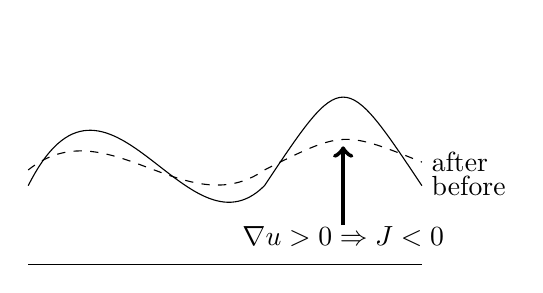
\begin{tikzpicture}
  \draw (0,1) .. controls (1,3) and (2,0) .. (3,1) .. controls (4,2.5) .. (5,1); % avant
  \draw[dashed] (0,1.2) .. controls (1,2) and (2,0.5) .. (3,1.2) ..controls (4,1.7) .. (5,1.3); %apres
  \draw (0,0) -- (5,0);
  \draw (5,1) node[right]{\text{before}};
  \draw (5,1.3) node[right]{\text{after}};
  \draw[ultra thick, ->] (4,0.5) -- (4,1.5);
  \draw (4,0.6) node[below]
  {$\nabla u > 0 \Rightarrow J<0$};
\end{tikzpicture}
    \caption{Before and after diffusion}
    \label{fig-diffusion}
\end{figure}


\subsection{Analysis of  \texorpdfstring{$\partial_t u = \kappa \partial_{xx} u$ in $(0,1)$}{diffusion equation}}

\begin{equation}
	\left\lbrace
	\begin{array}[]{rcll}
		\partial_t u &=& \kappa \partial_{xx} u
		& t>0 \, x\in (0,1)\\
		u(0,x) &=& u_0 (x) & x\in (0,1) \\
		u(t,0) &=& 0&\\
		u(t,1) &=& 0& \text{Homogeneous Dirichlet conditions}
	\end{array}\right.
\end{equation}

For simplicity, assume that $u_0(0) = u_0(1) = 0$.

\begin{rem}
	It is also natural to consider \definition{homogeneous
	Neumann boundary conditions}.
	$$\partial_x u(t,0) = 0 = \partial_x u(t,1)$$
	or 
	$$J(t,0) = 0 = J(t,1)$$.
	This is the adiabatique assumtion.
\end{rem}

We will study this initial bounding PDE problem with the help
of Fourier series. Ideas are

\begin{itemize}
	\item $e^{-\kappa k^2\pi^2 t}\sin(k\pi x)$ is a 
		solution to 
		\begin{equation}
	\left\lbrace
	\begin{array}[]{rcll}
		\partial_t u &=& \kappa \partial_{xx} u
		& t>0 \, x\in (0,1)\\
		u(0,x) &=& \sin(k\pi x) & x\in (0,1) \\
		u(t,0) &=& 0&\\
		u(t,1) &=& 0& 
	\end{array}\right.
\end{equation}
\item  The problem is linear, thus 
	$$u = \sum_{k=1}^l u_k e^{-\kappa k^2\pi^2 t}\sin(k\pi x)$$
	is solution to 
\begin{equation}
	\left\lbrace
	\begin{array}[]{rcll}
		\partial_t u &=& \kappa \partial_{xx} u
		& t>0 \, x\in (0,1)\\
		u(0,x) &=& \sum_{k=1}^l u_k 
		\sin(k\pi x) & x\in (0,1) \\
		u(t,0) &=& 0&\\
		u(t,1) &=& 0& 
	\end{array}\right.
\end{equation}.
\end{itemize}

\begin{lem}
	$\left( \sqrt{2} \sin(k\pi x) \right)_{k\in\N}$ is a 
	Hilbertian basis of $L^2(0,1)$.
\end{lem}

\begin{proof}
	See my lecture notes.
	(It is a consequence of the Fejer lemma for
	$\left( e^{2i\pi kx}\right)_{k\in\Z}$.)
\end{proof}

Any $u\in L^2(0,1)$ can be express as 
$$u(\cdot) = \sum_{k\in\N^*} \hat{u}(k) \sin(k\pi\cdot)$$
\footnote{it is an equality in $L^2$} with
$\hat{u}(k) = \sqrt{2} \int_0^1 u(x)\sin(k\pi x) \text{d}x$.
$$\sum_{k\in\N^*} \hat{u}(k) \sin(k\pi\cdot)
\xrightarrow{l\to\infty, L^2} u$$
Thus if $u_0\in L^2(0,1)$,
$$u_0 = \sqrt{2} \sum_{k\in\N^*} \hat{u_0}(k) \sin(k\pi\cdot)$$
We have a candidate to be solution
$$u(t,\cdot) = \sqrt{2} \sum_{k\in\N^*} e^{-\kappa k^2\pi^2 t}
\hat{u_0}(k) \sin(k\pi\cdot)$$.

\begin{prop}
	Under smoothness assumption on $u_0$,
	\begin{equation}
	\left\lbrace
	\begin{array}[]{ll}
		\partial_t u = \kappa \partial_{xx} u
		& t>0 \, x\in (0,1)\\
		u(0,x) = \sum_{k=1}^l u_k 
		\sin(k\pi x) & x\in (0,1) \\
		u(t,0) = u(t,1) = 0 & 
	\end{array}\right.
\end{equation}.
admits a unique solution.
\end{prop}

\begin{proof}
	For a more complet proof, see lecture notes.
\begin{itemize}
	\item Uniqueness:
	If the solution is in $L^2(0,1)$ for any time,
	let us denote 
	$\hat{u}(k) = \sqrt{2} \int_0^1 u(x)\sin(k\pi x) \text{d}x$. 
	And $\partial_t u = \kappa \partial_{xx} u$ becomes 
	$\hat{u}^\prime(t) = \kappa \hat{\partial_{xx}u} (k)$.
\begin{lem}
	Consider $g\in \mathcal{C}^2([0,1])$ such that 
	$g(0) = g(1) =0$. Then we have
	$\hat{g^{\prime\prime}}(k) = -k^2\pi^2 \hat{g}(k)$.
\end{lem}
\begin{proof}
	\begin{align*}
		\hat{g^{\prime\prime}}(k) &= \sqrt{2} \int_0^1
		g^{\prime\prime}(x)\sin(k\pi x) \text{d}x\\
		&=  \sqrt{2} \left[ 
			\underbrace{\left[ 
			g^\prime(x)\sin(k\pi x)\right]_0^1}_{=0}
			-k\pi\int_0^1 g^\prime(x)\cos(k\pi x)\text{d}x
	\right]\\
	&= -k\pi\sqrt{2} \left[ 
			\underbrace{\left[ 
			g(x)\cos(k\pi x)\right]_0^1}_{=0}
			+k\pi\int_0^1 g(x)\sin(k\pi x)\text{d}x
	\right]\\
	&= -k^2 \pi^2 \hat{g}(k)
\end{align*} 
\end{proof}
Thus 
\begin{align*}
	\hat{u}(k)^\prime (t) &=  -\kappa k^2 \pi^2 \hat{u}(k)(t)\\
	\Rightarrow \hat{u}(k)(t) &=\hat{u}(k)(0)
	e^{-\kappa k^2\pi^2 t }
\end{align*}.

\item To prove that
$u(t,x) = \sqrt{2} \sum e^{-\kappa k^2\pi^2 t}
\hat{u_0}(k) \sin(k\pi x)$ is a solution, one only has to 
prove that its is a function and is differentiable in time,
twice differentiable in space and such that it satisfies the
equation $\partial_t u = \kappa \partial_{xx} u$.
\begin{rem}
	Important point: $\kappa >0$, so that
	$e^{-\kappa k^2\pi^2 t}$ is rapidly decreasing.
\end{rem}
\end{itemize}
\end{proof}

The same method can be applied to prove the well-posedness of
\begin{equation}
	\left\lbrace
	\begin{array}[]{l}
		\partial_t u = \kappa \partial_{xx} u + f\\
		u(0,x) = u_0(x)  \\
		u(t,0) = u(t,1) = 0 
	\end{array}\right.
\end{equation}
where $f$ is a given function.

\begin{rem}
\begin{equation}
	\left\lbrace
	\begin{array}[]{l}
		\partial_t u = \kappa \partial_{xx} u + f\\
		u(0,x) = u_0(x)  \\
		\partial_x u(t,0) = \partial_x u(t,1) = 0 
	\end{array}\right.
\end{equation}
can be solved with the Hilbertian basis
$\left( 1,\left( \sqrt{2}\cos(k\pi x) \right)_{k\in\N^*} \right)$.
\end{rem}

\subsection{The maximal principle}

\begin{theo}
	Consider the unique solution $u$ to
\begin{equation}
	\left\lbrace
	\begin{array}[]{l}
		\partial_t u = \kappa \partial_{xx} u + f\\
		u(0,\cdot) = u_0 \text{ smooth } 
		u_0(0) = u_0(1) = 0\\
		u(t,0) = u(t,1) = 0 
	\end{array}\right.
\end{equation}
It satifies, for any $T>0$,
$$U = \max_{t\in [0,T]\, x\in(0,1)} u(t,x) = \max_{x\in (0,1)}
u_0(x)$$.
\end{theo}

\begin{proof}
	Idea of the proof: consider $(t,x)$ such that 
	$u(t,x) = \max_{s,y} u(s,y) = U$. Then
	$\partial_{xx}u(t,x) \le 0$ thus $\partial_t u(t,x)\le 0$
	($u$ was larger before).

	Rigourously, consider 
	$$v(t,x) = u(t,x)e^{\lambda t}$$
	for $\lambda \in\R$.
	We have
	\begin{align*}
		\partial_t v &= \partial_t u e^{\lambda t}
		+\lambda u e^{\lambda t}\\
		&= \kappa \partial_{xx} u e^{\lambda t} + \lambda v\\
		&= \kappa \partial_{xx} v + \lambda v
	\end{align*}
	then
\begin{equation}
	\left\lbrace
	\begin{array}[]{l}
		\partial_t v = \kappa \partial_{xx} v + 
		\lambda v\\
		v(0,\cdot) = u_0 \\
		v(t,0) = v(t,1) = 0 
	\end{array}\right.
\end{equation}
	Let us prove the theorem for $v$!
	Denote $V =  \max_{t\in [0,T]\, x\in(0,1)} v(t,x)  $
\begin{itemize}
\item Assume that $V = v(t_0,x_0)$ for 
	$(t_0,x_0)\in (0,T)\times [0,1]$.
\begin{itemize}
	\item If $x_0 = 0$ or $1$, $V=0$.
	\item If $x_0\in (0,1)$, $\partial_t v(t_0,x_0) = 0 =
		\partial_x v(t_0,x_0) $ and 
		$\partial_{xx} v(t_0,x_0) \le 0$.
		Since we have 
		$\partial_t v = \kappa \partial_{xx} v + \lambda v$,
		$ \lambda v(t_0,x_0) = - \kappa \partial_{xx}
		v(t_0,x_0) \ge 0$.
		Consider $\lambda >0$ then $v(t_0,x_0)\le 0$.
		Conclusion: $V\le 0$ if 
		$(t_0,x_0)\in (0,T)\times [0,1]$.
\end{itemize}
\item Assume that $V = v(T,x_0)$.
\begin{itemize}
	\item If $x_0 = 0$ or $1$, $V=0$.
	\item if not, 	$\partial_{xx} v(T,x_0) \le 0$ and
			$\partial_t v(T,x_0) \ge 0$.
	From $\partial_t v = \kappa \partial_{xx} v + \lambda v$,
	we deduce with $\lambda <0$ that $\partial_t v(T,x_0)\ge 0$.

\end{itemize}
\end{itemize}
Conclusion: if $t_0>0$, $V\le 0$.
But $\max_{y}u_0(y) \ge 0$. Thus, the maximum value is attained at
time $t=0$. $u(t,x) = v(t,x)e^{-\lambda t}$. When $\lambda\to 0^-$,
we observe that $u$ satisfies the maximum principle.
\end{proof}

Another proof of the maximum priciple:
\begin{proof}
	Consider $S: \R\rightarrow\R$, $S\in \mathcal{C}(\R)$ convex.
\begin{align*}
	& S^\prime(u) \partial_t u = \kappa S^\prime(u) 
	\partial_{xx} u \\
	& \partial_t S(u) = \kappa \partial_x(S(u)\partial_x u )
	- \underbrace{\kappa}_{\ge 0} 
	\underbrace{s^{\prime\prime}(u)}_{\ge 0} 
	\underbrace{\partial_x u}_{\ge 0} 
\end{align*}
Thus, $$\partial_t S(u) \le \kappa \partial_{xx}(S(u))$$
and
\begin{align*}
	& \int_0^1 \int_0^t \partial_t S(u) \text{d}s \text{d}x
	\le \kappa \int_0^1 \int_0^t \partial_{xx}S(u) 
	\text{d}s \text{d}x\\
	& \int_0^1 S(u(t,x)) \text{d}x 
	-  \int_0^1 S(u_0(x)) \text{d}x 
	\le \kappa \int_0^t\left[  \partial_x(S(u(s,1))) 
	- \partial_x(S(u(s,0))) \right]	\text{d}s
\end{align*}
Choose $S$,
% image
\begin{equation}
	S(u) = \left\lbrace 
	\begin{array}[]{ll}
		0 & \text{ if } u\le M = \max_x u_0(x)\\
		(u-M)^3  & \text{ if } u>M 
	\end{array}\right.
\end{equation}
is convex and in $\mathcal{C}^2$.

With this $S$, $S\circ u_0 = 0$. Thus,
$$\int_0^1 S(u(t,x)) \text{d}x 
\le \kappa \int_0^t\left[ S^\prime(\underbrace{u(s,1)}_{=0})
\partial_x u(s,1) - S^\prime(\underbrace{u(s,0)}_{=0})
\partial_x u(s,0) \right]	\text{d}s $$
and as $S^\prime(0) = 0$,
$$\int_0^1 S(u(t,x)) \text{d}x \le 0$$.
$S\circ u$ is non negative. Thus, $S\circ u (t,x) = 0$ (almost)
everywhere.
Finally, $u(t,x)\le M $ for all $x$.
\end{proof}

\begin{rem}
	This proof also works for homogeneous Neumann consitions.
	In fact, only parts that differ is that we have 
$$\int_0^1 S(u(t,x)) \text{d}x 
\le \kappa \int_0^t\left[ S^\prime(u(s,1))
\underbrace{\partial_x u(s,1)}_{=0} - S^\prime(u(s,0))
\underbrace{\partial_x u(s,0)}_{=0} \right]\text{d}s $$.
\end{rem}

\subsection{Numerical approximation}

We want to approximate the solution to
\begin{equation}
	\left\lbrace
	\begin{array}[]{l}
		\partial_t u = \kappa \partial_{xx} u + f\\
		u(0,\cdot) = u_0 \\
		u(t,0) = u(t,1) = 0 
	\end{array}\right.
\end{equation}

We want to compute $u_j^n$ that will be approximate values of 
$u(t^n,x_j)$.
Let $J\in\N^*$, $\Delta x = \frac{1}{J+1}$,
$x_j = j\Delta x$ where $j=0,1,\cdots , J+1$.
% une image
Let $\Delta t > 0$, $t^n = n\Delta t$, $n\in\N$.
If $u$ is smooth,
\begin{align*}
	\frac{u(t^{n+1},x_j) - u(t^n,x_j)}{ \Delta t}
	&\sim \partial_t u(t^n,x_j)\\
	\frac{u(t^{n},x_j) - u(t^{n-1},x_j)}{ \Delta t}
	&\sim \partial_t u(t^n,x_j)\\
	\frac{\partial_x u(t^{n},x_{j+\frac{ \Delta x}{2}}) 
	-\partial_x u(t^{n},x_{j-\frac{ \Delta x}{2}})}{ \Delta x}
	&\sim \partial_{xx} u(t^n,x_j)\\
	\frac{u(t^{n},x_{j+1}) - u(t^{n},x_j)}{ \Delta x}
	&\sim \partial_x u(t^n,x_{j+\frac{ \Delta x}{2}})\\
	\frac{u(t^{n},x_{j}) - u(t^{n},x_{j-1})}{ \Delta x}
	&\sim \partial_x u(t^n,x_{j-\frac{ \Delta x}{2}})\\
	\text{Finally, }
	\frac{u(t^{n},x_{j+1}) -2u(t^{n},x_{j}) +u(t^{n},x_{j-1}) 
	}{ \Delta x^2}
	& \sim \partial_{xx} u(t^n,x_j)
\end{align*}
(To be prove at the end in the consistency statement!)

We have at least two schemes:
\begin{equation}
	\tag{$\mathcal{E}$}
	\frac{u({n+1}_j - u^n_j}{ \Delta t} = \kappa
	\frac{u^{n}_{j+1} -2u^{n}_{j} +u^{n}_{j-1}}{\Delta x^2}
	+f(t^n,x_j)
	\label{eq-diffusion-explicit}
\end{equation}
\begin{equation}
	\tag{$\mathcal{I}$}
	\frac{u({n+1}_j - u^n_j}{ \Delta t} = \kappa
	\frac{u^{n+1}_{j+1} -2u^{n+1}_{j} +u^{n+1}_{j-1}}{\Delta x^2}
	+f(t^{n+1},x_j)
	\label{eq-diffusion-implicit}
\end{equation}

Precisely, the explicit scheme is

\begin{equation}
	\tag{$\mathcal{E}$}
	\left\lbrace 
	\begin{array}[]{ll}
	\frac{u({n+1}_j - u^n_j}{ \Delta t} = \kappa
	\frac{u^{n}_{j+1} -2u^{n}_{j} +u^{n}_{j-1}}{\Delta x^2}
	+f(t^n,x_j)
	& n\in\N \, j=1,\cdots , J\\
	u^n_0 =u^n_{j+1} = 0 & n\in\N \\
	u^0_j = u_0(x_j) & j=1,\cdots , J
	\end{array}\right.
	\label{eq-diffusion-explicitP}
\end{equation}

\begin{theo}
	Assume that $\kappa\Delta t\le \frac{ \Delta x^2}{2}$.
	Then if $(u^n_j)$ is defined by \eqref{eq-diffusion-explicitP},
	$$\sup_j \vert u(t^n,x_j)\vert \le 
	C t^n (\Delta t +\Delta x^2)$$
	if $u\in \mathcal{C}^{2,4}_b(\R^+, [0,1])$.
	(The scheme is fist order in $\Delta t$ and second order
	in $\Delta x$ convergent.)
\end{theo}

\begin{proof}
\begin{itemize}
\item Consistency:
	\begin{equation}
		\varepsilon^n_j = 
	\frac{u(t^{n+1},x_j) - u(t^n,x_j)}{ \Delta t} - \kappa
	\frac{u(t^{n},x_{j+1}) -2u(t^{n},x_{j}) 
	+u(t^{n},x_{j-1})}{\Delta x^2}
	- f(t^n,x_j)
		%\label{}
	\end{equation}
If $u\in \mathcal{C}^{2,4}_b(\R^+, [0,1])$, we can prove that
$\vert\varepsilon\vert\le C(\Delta t+ \Delta x^2)$.
Indeed,
\begin{align*}
	&\frac{u(t^{n+1},x_j) - u(t^n,x_j)}{ \Delta t}
	= \partial_t u(t^n,x_j) + \mathcal{0}(\Delta t)\\
	u(t^{n},x_{j+1}) &= u(t^{n},x_{j}) 
	+ \Delta x \partial_x u(t^n,x_{j})
	+ \frac{ \Delta x^2}{2} \partial_{xx} u(t^n,x_{j})
	+ \frac{ \Delta x^3}{6} \partial_{xxx} u(t^n,x_{j})
	+ \mathcal{0}(\Delta x^4)\\
	u(t^{n},x_{j-1}) &= u(t^{n},x_{j}) 
	- \Delta x \partial_x u(t^n,x_{j})
	+ \frac{ \Delta x^2}{2} \partial_{xx} u(t^n,x_{j})
	- \frac{ \Delta x^3}{6} \partial_{xxx} u(t^n,x_{j})
	+ \mathcal{0}(\Delta x^4)\\
	\text{Thus, }
	&\frac{u(t^{n},x_{j+1}) -2u(t^{n},x_{j}) +u(t^{n},x_{j-1}) 
	}{ \Delta x^2}
	= \partial_{xx} u(t^n,x_j)+ \mathcal{0}(\Delta x^2)
\end{align*}
and
	\begin{equation}
		\varepsilon^n_j = 
		\partial_t u(t^n,x_j) 
		-\kappa \partial_{xx} u(t^n,x_j) -f(t^n,x_j)
		+ \mathcal{0}(\Delta t)+ \mathcal{0}(\Delta x^2)
	\end{equation}
\item Stability:
	Define
	\begin{equation}
		e^n_j = u^n_j - u(t^n,x_j) 
	\end{equation}.
We have
\begin{align*}
	&\frac{e^{n+1}_j - e^n_j}{ \Delta t} - \kappa
	\frac{e^{n}_{j+1} -2e^{n}_{j} +e^{n}_{j-1}}{\Delta x^2}
	= -\varepsilon^n_j\\
	& e^{n+1}_j = e^n_j\left( 1 -
	\frac{2\kappa\Delta t}{\Delta x^2} \right) 
	+ e^{n}_{j+1} \frac{\kappa\Delta t}{\Delta x^2}  
	+ e^{n}_{j-1} \frac{\kappa\Delta t}{\Delta x^2} 
 	- \Delta t \varepsilon^n_j\\
	\text{Thus, }
	&\vert e^{n+1}_j\vert = \vert  e^n_j \vert  \left( 1 -
	\frac{2\kappa\Delta t}{\Delta x^2} \right) 
	+ \vert e^{n}_{j+1}\vert  \frac{\kappa\Delta t}{\Delta x^2}  
	+ \vert e^{n}_{j-1}\vert  \frac{\kappa\Delta t}{\Delta x^2} 
 	+ \Delta t \vert  \varepsilon^n_j\vert \\
	&\le \max_{j=1,\cdots, J} \vert e^n_j\vert 
	+ \Delta t C (\Delta t +\Delta x^2)\\
	\text{If } 	\frac{2\kappa\Delta t}{\Delta x^2} \le 1
	&\le \max_{j=1,\cdots, J} \underbrace{\vert e^0_j\vert}_{=0}
	+ \underbrace{(n+1)\Delta t}_{t^{n+1}}
	C (\Delta t +\Delta x^2)
\end{align*}
\end{itemize}
\end{proof}


% COURS DU 21/11/2018

\chapter{Perfect fluid}
\footnote{Fluides parfaits}

On considère un fluide occupant $\R^d$ ($d=1,2,3$) ou
$\Omega\in\R^d$ de densité $\rho(t,x)$ (densité
volumique de masse) at time $t\in\R$, position $x\in\R^d$
and velocity $u(t,x)\in\R^d$.

We will derive equations on $\rho$ and $u$ (at least)
allowing to know (compute) $\rho(t,x)$ and $u(t,x)$
knowing some initial conditions, e.g.  $\rho(0,x)$ and
$u(0,x)$ for all $x$.

The first physical principle we can use to obtain an
equation is the conservation of mass.
\begin{equation}
	\partial_t\rho + \nabla(\rho u ) = 0
	\quad (t,x)\in\R\times\Omega
%	\label{}
\end{equation}

Indeed, let $\omega(t)$ be a material volume.
\begin{equation}
	\omega(t) = \left\{ 
		x\in\R^d \vert \exists y\in\R^d 
	\text{ s.t.}
		\begin{array}[ ]{cl}
		\cdot & y= \omega(0) \\
		\cdot & x =X(t,y)
		\end{array} 
	\text{ where } \left\lbrace
		\begin{array}[ ]{cl}
		& \partial_t X(t,y) = u(t,X(t,y))\\
		& X(o,y) = y	
		\end{array} \right.
	\right\}
	%\label{}
\end{equation}

Then
\begin{align*}
	0 = &
	\frac{\text{d}}{\text{d}t} \int_{\omega(t)}
	\rho(t,y) \text{d} y \\
	&= \int_{\omega(t)}\partial_t\rho(t,y) \text{d}y +
	\int_{\partial\omega(t)}\rho u \cdot n\text{d}y\\
	&= \int_{\omega(t)}\partial_t\rho +
	\int_{\omega(t)}\nabla\cdot(\rho u )\\
	&= \int_{\omega(t)}\left( \partial_t\rho +
	\nabla\cdot(\rho u ) \right)\\
	\footnote{ physically\dots} \Rightarrow & 
	\partial_t\rho +\nabla\cdot(\rho u ) = 0\in \R
\end{align*}

But, here $u$ is not a given vector field.
There lacks at least une equation (in $\R^d$).
(We have $(\rho, u)\in\R^{d+1}$ as unknowns.)

Newton's second law provides another equation.
$$m \dot{u} = m \ddot{x}(t) = F$$
for a particle with constant mass, position $x$,
submitted to its force $F$.

Applying this to material volume $\omega(t)$, we get
\begin{equation}
	\frac{\text{d}}{\text{d}t}
	\underbrace{\int_{\omega(t)}
	\rho(t,y)u(t,y) \text{d} y }_{
		\text{ impulse of } \omega(t)} =
	\text{ forces acting on } \omega(t)
%	\label{}
\end{equation}.

\paragraph{Forces acting on $\omega(t)$}
\begin{itemize}
	\item external volume forces $f$: 
		(for example, the gravity force)
	\item thers is no internal forces thanks to 
		Newton's third law: action-reaction
		principle.
	\item surface forces $f_\sigma$ acting on 
		$\partial\omega(t)$ thus we have
$$\int_{\omega(t)}\partial_t(\rho u) +
\int_{\partial\omega(t)}(\rho u)(u\cdot n)\text{d}\sigma
= \frac{\text{d}}{\text{d}t} \int_{\omega(t)}(\rho u) \\
= \int_{\omega(t)} f + \int_{\partial\omega(t)} f_\sigma$$.
\footnote{ $(\rho u )(u\cdot n) $ is the 
vector with component $(\rho u )_i\cdot 
(u\cdot n) \quad i = 1,\cdots , d$. }
\end{itemize}

Furthermore, we have
\begin{lem}
\begin{equation}
	\int_{\partial\omega(t)}(\rho u )(u\cdot n) =
	\int_{\omega(t)}\nabla\cdot (\rho u\otimes u) 
	\label{lemme-inter-1}
\end{equation}
where	
\begin{align*}
	\rho u \otimes u &= \rho( u \otimes u)\\
	u\otimes u(t,x) & \in \mathcal{M}_d(\R)
	\text{ with } (u\otimes u)_{i,j} = u_iu_j
\end{align*}
If $M$ is a matrix field then $\nabla\cdot M $ is the
vector field where the $i$-th component is the divergence 
of the corresponding line of $M$.
$$(\nabla \cdot M)_i = \sum_{j=1}^d \partial_jM_{i,j}$$.
Thus,
$(\nabla\cdot \rho u\otimes u)_i = \sum_{j=1}^d \partial_j
(\rho u_iu_j)$.
\end{lem}

\begin{proof}
	Let us prove \ref{lemme-inter-1}.
	For any $i=1,\cdots ,d$,
	$$(\int_{\partial\omega(t)}(\rho u )(u\cdot n))_i
	=\int_{\partial\omega(t)} \rho u_i(u\cdot n)
	=\int_{\partial\omega(t)} \nabla(\rho u_i u)
	=\int_{\partial\omega(t)} \sum_{j=1}^d 
	\partial_j(\rho u_iu_j)
	=(\int_{\omega(t)}\nabla\cdot (\rho u\otimes u) )_i
	$$.
\end{proof}

Thus, we have 
\begin{equation}
	\int_{\omega(t)}\partial_t(\rho u) +
	\nabla\cdot (\rho u\otimes u) 
= \int_{\omega(t)} f + \int_{\partial\omega(t)} f_\sigma
	%\label{}
\end{equation}.

\begin{definition}
	Let $x\in \Omega$ (in the fluid!). Let $n\in\R^d$
	be a normed vector, $\varepsilon >0$ and 
	$D(x,n,\varepsilon)$ be the disk centered at $x$,
	orthogonal to $n$ with surface $\varepsilon$.

	%%%pictures%%%%%%

	Assume that the force $F(x,n,\varepsilon)$
	exerted by the fluid on the 
	side where $n$ points over $D(x,n,\varepsilon)$
\begin{itemize}
	\item is parallel to $n$ and
	\item is equivalent, as $\varepsilon\to 0$, to
		$\varepsilon p(x) n$.
		$$\frac{ F(x,n,\varepsilon)}{ \varepsilon}
		\xrightarrow{}_{\varepsilon\to 0^+}
		-p(x) n$$
\end{itemize}
Then the fluid is called \definition{perfect}, and the
scalar $p(x)$ is called its \definition{pressure}.
\end{definition}

In a perfect fluid with pressure p(x),
\begin{equation}
	\int_{\partial\omega(t)}f_\sigma =
	\int_{\partial\omega(t)}-pn
	%\label{}
\end{equation}.
Assume that the fluid is perfect with pressure $p(t,x)$.
We have 
$$\int_{\omega(t)}\partial_t(\rho u)+\nabla(\rho u\otimes u)
= \int_{\omega(t)} f - \int_{\partial\omega(t)} p n
= \int_{\omega(t)} f - \underbrace{\int_{\omega(t)} \nabla p
}_{\int_{\omega(t)} \nabla\cdot (p I)}
$$.
Thus, for any $\omega(t)$,
\begin{equation}
	\int_{\omega(t)}\left( 
	\partial_t(\rho u)+\nabla(\rho u\otimes u)
	+  \nabla p - f \right) = 0
	%\label{}
\end{equation}
and 
\begin{equation}
	\partial_t(\rho u)+\nabla(\rho u\otimes u)
	+  \nabla p = f \in\R^d
	%\label{}
\end{equation}
or
\begin{equation}
	\partial_t(\rho u)+\nabla(\rho u\otimes u + pI)
	= f \in\R^d
	%\label{}
\end{equation}.

Usually, $f$ is known. For example,
\begin{ex}
	If $f$ is the gravity force (assumed to be constant),
	$f= \rho g$. And
	\begin{equation}
		\left\lbrace
		\begin{array}[]{l}
			\partial_t \rho +\nabla(\rho u )=0\\
			\partial_t(\rho u ) +\nabla
			(\rho u\otimes u ) +\nabla p
			= \rho g
		\end{array}\right.
	\end{equation}
	is a system of $d+1$ equations and $d+2$ unknowns.
\end{ex}

\paragraph{Ways to close the system}

\begin{itemize}
	\item Assume that $p=p(\rho)$
		\definition{Barotropic gaz}
\begin{ex}
	\begin{itemize}
		\item \definition{Isothermal gaz}:
			$p=C\rho$.
		\item \definition{Adiabatic gaz}:
			$p=C\rho^\gamma$ with $\gamma >1$.
	\end{itemize}
\end{ex}
	In this case, if $d=1$ and neglecting external
	forces, we have
	\begin{equation}
		\left\lbrace
		\begin{array}[]{l}
			\partial_t\rho+\partial_x(\rho u )=0\\
			\partial_t(\rho u ) + \partial_x
			(\rho u^2 + p(\rho)) = 0
		\end{array}\right.
	\end{equation}
	This is a hyperbolic system, if $p$ is an increasing
	function of $\rho$.
	We also remark that
\begin{equation}
	\partial_t \left(
	\begin{array}[]{c}
		\rho \\
		\rho u
	\end{array} \right)
	+ \partial_x F(\rho, \rho u ) = 0
	\quad \text{ with }
 	F(\rho, \rho u ) = 
	\left(
	\begin{array}[]{c}
		\rho u \\
		\rho u^2 + p(\rho)
	\end{array} \right)
\end{equation}

\begin{equation}
	\underbrace{\Leftrightarrow}_{\text{
	if the solution is smooth}} 
	\partial_t \left(
	\begin{array}[]{c}
		\rho \\
		\rho u
	\end{array} \right)
	+ \underbrace{\nabla_{\rho, \rho u} F(\rho, \rho u )
}_{2\times 2 \text{ matrix, }\R \text{-diagonalizable}}
	\partial_x \left(
	\begin{array}[]{c}
		\rho \\
		\rho u
	\end{array} \right)
	= 0
\end{equation}

\item If the pressure also depends on the temperature $T$,
	we have
	\begin{equation}
		\left\lbrace
		\begin{array}[]{l}
			\partial_t \rho +\nabla(\rho u )=0\\
			\partial_t(\rho u ) +\nabla
			(\rho u\otimes u ) +\nabla p(\rho,T)I
			= 0
		\end{array}\right.
	\end{equation}.
	We need another equation. What is usually done is 
	is to define the total energy 
	$$e(t,x) = \frac{1}{2} \vert u\vert^2 + \varepsilon$$
	where $\varepsilon$ is the internal energy.
	It is commmonly assumed that $\varepsilon = c_vT$
	($c_v$ is known.) 
	We have a physical priciple
	\definition{ conservation of total energy}
	\begin{equation}
		\partial (\rho e) +\nabla (\rho eu +
		\underbrace{pu}_{\text{power of pressure}})
		= \underbrace{fu}_{\text{power of
		external forces}}
		%\label{}
	\end{equation}
	then
	$$p = p(\rho,T)=p(\rho, \frac{ \varepsilon}{c_v})
	= p(\rho, \frac{e - \frac{ \vert u\vert^2}{2}}{c_v})
	= \tilde{p} (\rho, u, e)$$
	and the system is closed.
\begin{ex}
	$$p=\tilde{p}(\rho, u ,e) = (\gamma-1)\rho \varepsilon
	= (\gamma-1)\rho(e - \frac{ \vert u\vert^2}{2}) $$
	$$\Leftrightarrow PV = nRT$$
	(\definition{ Ideal gas law})

	With $\gamma >1$, the system is hyperbolic and has
	three different eigenvalues.
\end{ex}

\begin{rem}
	$d=1$, \definition{ Isobaric(compressible) gas}
	with $p=p(\rho)$.
	\begin{equation}
		\left\lbrace
		\begin{array}[]{l}
			\partial_t\rho+\partial_x(\rho u )=0\\
			\partial_t(\rho u ) + \partial_x
			(\rho u^2 + p(\rho)) = 0
		\end{array}\right.
	\end{equation}
	If $\rho$, $u$ are smooth, we have
	\begin{equation}
		\left\lbrace
		\begin{array}[]{l}
			\partial_t\rho+\partial_x(\rho u )=0\\
			\rho\partial_t u + \underbrace{
			u\partial_t\rho + u \partial_x\rho 
			u}_{ = 0} + \rho u  \partial_x u 
			+ \partial_x p= 0
		\end{array}\right.
	\end{equation}
	thus 
	$$\rho(\underbrace{ \partial_t u + u\partial_x u}_{
	\text{terms of Burger's equation}}+\partial_x p= 0$$.
\end{rem}

\item Assume \textbf{incompressibility} of the fluid: the
	volume of a material volume $\omega(t)$ does not 
	depend on time.
	$$\frac{\text{d}}{\text{d}t}(\int_{\omega(t)} 1 
	\text{d}x) = 0 =\int_{\omega(t)} \underbrace{
	\partial_t 1}_{=0} + \int_{\partial\omega(t)} 1 u 
	\cdot n = \int_{\omega(t)} \nabla\cdot u$$.
	Thus $\nabla\cdot u = 0$. ($\nabla_x u(t,x) = 0\,
	\forall t, x$.)
	Finally,
	\begin{equation}
		\left\lbrace
		\begin{array}[]{l}
			\partial_t \rho +\nabla(\rho u )=0\\
			\partial_t(\rho u ) +\nabla
			(\rho u\otimes u ) +\nabla p
			= 0\\
			\nabla\cdot u = 0
		\end{array}\right.
	\end{equation}.
\begin{prop}
	In a perfect incompressible fluid, we have
	\begin{equation}
		\left\lbrace
		\begin{array}[]{l}
			\partial_t \rho + u \nabla\rho=0\\
			\partial_t(\rho u ) +\nabla
			(\rho u\otimes u ) +\nabla p
			= f\\
			\nabla\cdot u = 0
		\end{array}\right.
	\end{equation}.
	where $(u\cdot\nabla)$ is defined as
	$$((u\cdot\nabla)v)_i 
	=\sum_{j=1}^d u_j\partial_jv_i
	= (\nabla v \cdot u )_i$$
	thus
	$((u\cdot\nabla)u)_i 
	=\sum_{j=1}^d u_j\partial_ju_i$.
\end{prop}

\begin{proof}
	First equation:
	$$\partial_t\rho +\nabla(\rho u) = 0 
	= \partial_t\rho + u\nabla\rho + \rho
	\underbrace{\nabla u}_{=0}$$

	Second equation:
	First remark that if $d=1$, this writes
	$$\rho(\partial_x u + u\partial_x u ) + \partial_x p
	= f $$
	that we already derived.
	We start with 
	$$\partial_t(\rho u) +\nabla\rho u\otimes u +
	\nabla p = f$$.
	For the fisrt term, $\partial_t(\rho u) =
	\rho\partial_t u + u\partial_t\rho$.
	Let us decompose $\nabla\cdot\rho u\otimes u$
\begin{align*}
	(\nabla\rho u\otimes u)_i &= 
	\sum_{j=1}^d \partial_j(\rho u_iu_j)\\
	&= \sum_{j=1}^d \rho u_j\partial_ju_i +
	\sum_{j=1}^d  u_i\partial_j(\rho u_j)\\
	&= (\rho(u\cdot\nabla)u)_i + u_i \sum_{j=1}^d 
	\partial_j(\rho u_j)\\
	&= (\rho(u\cdot\nabla)u)_i+(\nabla\cdot(\rho u)u)_i\\
        \Rightarrow \nabla\rho u\otimes u &=
	\rho(u\cdot\nabla)u+\nabla\cdot(\rho u)u
\end{align*}
Thus,
\begin{align*}
	f &=\partial_t(\rho u)+\nabla\rho u\otimes u 
	+\nabla p\\
	&= \rho\partial_t u + \underbrace{u\partial_t\rho
	+ u\nabla(\rho u)}_{=0} + \rho(u\cdot\nabla)u 
	+\nabla p \\
	&= \rho(\partial_t u + u\nabla u ) + \nabla p 
\end{align*}
\end{proof}
\end{itemize}

\begin{rem}
	If $\rho \neq 0$, the impulse equation is often 
	written as 
	$$\partial_t u + (u\cdot \nabla )u + 
	\frac{\nabla p}{ \rho} = \frac{f}{ \rho}
	= g \quad \text{ if } f = \rho g$$.
\end{rem}

\begin{rem}
	The equation $\nabla u = 0 $ plays a particular 
	role. It is not an evolution equation.

	This can be seen as a constraint on the fluid.
	From this point of view, $p$ can be understood 
	as a Lagrange multiplier associated with this
	constraint. We will see it a bit more precisely 
	in similar context: Stokes equation.
\end{rem}





%%%%%%%%%%%%%%%%%%%%%%%% 
%%%%%% APPENDICES %%%%%% 
%%%%%%%%%%%%%%%%%%%%%%%% 
\begin{appendices}

\chapter{Answers to exercises}

\section{}\label{sec-ans-0912-1} \ref{sec-ans-0912-1}

\begin{proof}
Since we have 
$$V^{int} = \sum_{i<j} V(\vert x_j -x_i \vert)$$.
Then 

The notation in course are strange.
\end{proof}

\section{}
\label{ans1}

\theorem{Lemma} : if $\rho \in C^3_U(\R_{+} \times \R)$,
\begin{equation}
\exists C,\quad \vert \varepsilon_j^n \vert \le C (\Delta t + \Delta x^2)
\end{equation}  
with 
\begin{equation}
\varepsilon^n_j = \frac{\rho(t^{n+1},x_j)-\rho(t^n,x_j)}{\Delta t} + u\frac{\rho(t^{n},x_{j+1})-\rho(t^n,x_{j-1})}{2\Delta x}
\end{equation}

\begin{answer}
	With a Taylor expansion, we have:
\begin{align*}
	\rho(t^{n+1},x_j) - \rho(t^n,x_j) &=
	\Delta t \partial_t\rho(t^n,x_j) + \mathcal{O}(\Delta t^2)\\
	\rho(t^n,x_{j+1}) - \rho(t^n,x_j) &=
	\Delta x \partial_x\rho(t^n,x_j) +
	\frac{\Delta x^2}{2} \partial_x^2\rho(t^n,x_j) 
	+ \mathcal{O}(\Delta x^3)\\
	\rho(t^n,x_{j-1}) - \rho(t^n,x_j) &=
	-\Delta x \partial_x\rho(t^n,x_j) 
	+\frac{\Delta x^2}{2} \partial_x^2\rho(t^n,x_j) 
 	+ \mathcal{O}(\Delta x^3)
\end{align*}
By substracting the last two relations, we obtain:
\begin{align*}
	\rho(t^n,x_{j+1}) - \rho(t^n,x_{j-1}) &=
	2\Delta x \partial_x\rho(t^n,x_j) + \mathcal{O}(\Delta x^3)\\
\end{align*}
Thus,
\begin{align*}
	\varepsilon^n_j &= \partial_t\rho(t^n,x_j) + 
	\mathcal{O}(\Delta t) + u\partial_x\rho(t^n,x_j)
	+ \mathcal{O}(\Delta x^2)\\
	&= \mathcal{O}(\Delta t +\Delta x^2)
\end{align*}
Then we can conclude.
\end{answer}

\section{}
\label{ans3}

\begin{answer}[Verification]
\begin{eqnarray*}
e_j^{n+1} &=& 
\rho_j^n 
-u\frac{\Delta t}{2\Delta x}\left(\rho_{j+1}^n - \rho^n_{j-1}\right)
- \left(\rho(t^{n},x_j) -  u\frac{\Delta t}{2\Delta x}
(\rho(t^{n},x_{j+1})-\rho(t^n,x_{j-1}) 
+\Delta t\varepsilon^n_j  \right).\\
&=& e^n_j - u\frac{\Delta t}{2\Delta x} (e^n_{j+1} - e^n_{j-1}) 
- \Delta t \varepsilon^n_j
\end{eqnarray*}
\end{answer}

\section{Proof of discrete Gronwall Lemma} \label{ans4}
\begin{answer}
	Remark that $1+\Delta t \le e^{C\Delta t}$ (since $C\Delta t$
	is positive), then we can prove the implication by recurrence.
\end{answer}

\section{Lax-Wendroff scheme} \label{ans2}

\textbf{Exercise}. \\
The Lax-Wendroff scheme is :
\begin{equation}
\rho_j^{n+1} = \rho_j^{n} - \frac{\nu}{2}\left(\rho^n_{j+1} - \rho^n_{j-1} \right) + \frac{\nu^2}{2}\left(\rho^n_{j+1} - 2\rho^n_{j} + \rho^n_{j-1}\right)
\end{equation}
Prove that this scheme is $2^{nd}$ order (in $\Delta t$ and $\Delta x$) consistent.
Prove that the scheme is $\ell^2$-stable $\left(\Vert \rho^{n+1}\Vert_{\ell^2} \le \Vert \rho^{n}\Vert_{\ell^2}\right)$ \quad (and convergent) under the CFL condition $\nu \le 1$.

\begin{answer}
\underline{\textbf{Consistency:}}

	We define 
\begin{equation*}
\Delta t\varepsilon^n_j = \rho(t^{n+1},x_j) - \rho(t^n,x_j) + 
\frac{\nu}{2}\left(\rho(t^n,x_{j+1}) - \rho(t^n,x_{j-1}) \right) 
- \frac{\nu^2}{2}\left(\rho(t^n,x_{j+1}) - 2\rho(t^n,x_j) 
+ \rho(t^n,x_{j-1})\right)
\end{equation*}
With a Taylor expansion, we have:
\begin{align*}
	\rho(t^{n+1},x_j) - \rho(t^n,x_j) &=
	\Delta t \partial_t\rho(t^n,x_j) 
	+  \frac{ \Delta t^2}{2} \partial_t^2\rho(t^n,x_j) 
	\mathcal{O}(\Delta t^3)\\
	\rho(t^n,x_{j+1}) - \rho(t^n,x_j) &=
	\Delta x \partial_x\rho(t^n,x_j) 
	+ \frac{\Delta x^2}{2} \partial_x^2\rho(t^n,x_j) 
	+ \mathcal{O}(\Delta x^3)\\
	\rho(t^n,x_{j-1}) - \rho(t^n,x_j) &=
	-\Delta x \partial_x\rho(t^n,x_j)
	+ \frac{\Delta x^2}{2} \partial_x^2\rho(t^n,x_j) 
	+ \mathcal{O}(\Delta x^3)
\end{align*}
By summing and substracting the last two relations, we obtain:
\begin{align*}
	\rho(t^n,x_{j+1}) - \rho(t^n,x_{j-1}) &=
	2\Delta x \partial_x\rho(t^n,x_j) + \mathcal{O}(\Delta x^3)\\
	\rho(t^n,x_{j+1}) - 2\rho(t^n,x_j)+\rho(t^n,x_{j-1})  &=
	\Delta x^2\partial_x^2\rho(t^n,x_j)+\mathcal{O}(\Delta x^3)
\end{align*}
By deriving the equation with respect to $t$ and $x$, 
we will also have:
\begin{equation*}
	\partial_t^2 \rho = u^2\partial_x^2 \rho	
\end{equation*}.
Thus,
\begin{align*}
	\Delta t\varepsilon^n_j 
	&= \Delta t \partial_t\rho(t^n,x_j) 
	+  \frac{ \Delta t^2}{2} \partial_t^2\rho(t^n,x_j) + 
	\mathcal{O}(\Delta t^3) + \frac{\nu}{2}  \left( 2\Delta x
	\partial_x\rho(t^n,x_j) + \mathcal{O}(\Delta x^3) \right)
	- \frac{\nu^2}{2} \left( \Delta x^2\partial_x^2\rho(t^n,x_j)
	\mathcal{O}(\Delta x^3)\right)\\
	 &= \Delta t \left( \partial_t\rho(t^n,x_j) + 
	 u \partial_x\rho(t^n,x_j) \right)
	 +  \frac{ \Delta t^2}{2} \partial_t^2\rho(t^n,x_j) 
	 -\frac{u^2\Delta t^2}{2} \partial_x^2\rho(t^n,x_j)
	+ \mathcal{O}(\Delta t^3) + \mathcal{O}(\Delta t\Delta x^2) 
	+ \mathcal{O}(\Delta t^2 \Delta x)\\
	\varepsilon^n_j 
	&= \mathcal{O}(\Delta t^2) + \mathcal{O}(\Delta x^2) 
	+ \mathcal{O}(\Delta t \Delta x)
\end{align*}
Therefore, the scheme is consistent of order $2$.

\underline{\textbf{$\ell^2 $ stability:}}

Assume that $\rho^n_j\in\ell^2$ so we can define $\rho^n_\Delta\in L^2$
with the same definition as before.
Then, we have
\begin{equation*}
\rho^{n+1}_\Delta = \rho^n_\Delta - \frac{\nu}{2}\left(
\rho^n_\Delta(\cdot +\Delta x) - \rho^n_\Delta(\cdot -\Delta x) \right)+ \frac{\nu^2}{2}\left( \rho^n_\Delta(\cdot +\Delta x) 
-2 \rho^n_\Delta + \rho^n_\Delta(\cdot -\Delta x) \right)
\end{equation*}

Then
\begin{align*}
	\Vert \rho^{n+1}\Vert &= \frac{1}{\sqrt{\Delta x}}
	\Vert \rho^{n+1}_\Delta \Vert_{\ell^2} 
	= \frac{1}{\sqrt{\Delta x}}
	\Vert \hat{\rho^{n+1}_\Delta} \Vert_{L^2}\\
 	&= \frac{1}{\sqrt{\Delta x}} \Vert \hat{\rho^n_\Delta} 
	-\frac{\nu}{2}  \hat{\rho^n_\Delta} 
	\left( e^{ i\Delta x \xi} -  e^{-i\Delta x \xi} \right)
	+\frac{\nu^2}{2}  \hat{\rho^n_\Delta} 
	\left( e^{ i\Delta x \xi} +  e^{-i\Delta x \xi}-2 \right)
	\Vert_{L^2}\\
	&= \frac{1}{\sqrt{\Delta x}} \Vert \hat{\rho^n_\Delta} \Vert_{L^2}
	\Vert -\frac{\nu}{2} 
	\left( e^{ i\Delta x \xi} -  e^{-i\Delta x \xi} \right)
	+\frac{\nu^2}{2} \left( e^{ i\frac{\Delta x \xi}{2}} -  e^{-i\frac{\Delta x \xi}{2}} \right)^2 \Vert\\
	&= \frac{1}{\sqrt{\Delta x}} \Vert \hat{\rho^n_\Delta} \Vert_{L^2}
	\Vert 1 - i \nu \sin(\Delta x \xi)
	- 2 \nu^2  \sin^2(\frac{\Delta x \xi}{2})
	\Vert\\
	&= \frac{1}{\sqrt{\Delta x}} \Vert \hat{\rho^n_\Delta} \Vert_{L^2}
	\Vert (1 - 2 \nu^2  \sin^2(\frac{\Delta x \xi}{2}))^2
	+ \nu^2 \sin^2(\Delta x \xi)	\Vert\\
	&= \frac{1}{\sqrt{\Delta x}} \Vert \hat{\rho^n_\Delta} \Vert_{L^2}
	\Vert [1 - \nu^2 + \nu^2(1- 2\sin^2(\frac{\Delta x \xi}{2})]^2
	+ \nu^2 \sin^2(\Delta x \xi)	\Vert\\
	&= \frac{1}{\sqrt{\Delta x}} \Vert \hat{\rho^n_\Delta} \Vert_{L^2}
	\Vert (1 - \nu^2)^2 + 2(1 - \nu^2)\nu^2\cos(\Delta x \xi)
	+\nu^4\cos^2(\Delta x \xi) + \nu^2 \sin^2(\Delta x \xi)	\Vert\\
	&= \frac{1}{\sqrt{\Delta x}} \Vert \hat{\rho^n_\Delta} \Vert_{L^2}
	\Vert (1 - \nu^2)^2 + 2(1 - \nu^2)\nu^2
	+\nu^2	\Vert \text{ since } \mu^2 < 1 \Rightarrow \mu^4 < \mu^2\\
	&=\frac{1}{\sqrt{\Delta x}} \Vert \hat{\rho^n_\Delta} 
	\Vert_{L^2} = \Vert \rho^n\Vert  
\end{align*}
Thus $\Vert \rho^{n+1}\Vert \le  \Vert \rho^n\Vert $,
and we can conclude that the scheme is $\ell^2$ stable.
\end{answer}

\section{}  \label{sec-ans-1009-1}.

\begin{exercise}
	\begin{itemize}
\item Prove that 
	$\vert\varepsilon^n_j\vert\le C(\Delta t + \Delta x)$ if
	$\rho$ is smooth.
\item Prove the convergence of the scheme under the CFL condition.
	\end{itemize}
\end{exercise}

\begin{answer}
	With a Taylor expansion, we have:
\begin{align*}
	\rho(t^{n+1},x_j) - \rho(t^n,x_j) &=
	\Delta t \partial_t\rho(t^n,x_j) + \mathcal{O}(\Delta t^2)\\
	\rho(t^n,x_j) - \rho(t^n,x_{j-1})&=
	\Delta x \partial_x\rho(t^n,x_j) + \mathcal{O}(\Delta x^2)
\end{align*}
Thus,
\begin{align*}
	\varepsilon^n_j &= \partial_t\rho(t^n,x_j) + 
	\mathcal{O}(\Delta t) + u\partial_x\rho(t^n,x_j)
	+ \mathcal{O}(\Delta x)\\
	&= \mathcal{O}(\Delta t +\Delta x)
\end{align*}
Thus, we have the result.

Moreover, under the CFL condition, we have:
\begin{align*}
	\vert e^{n+1}_j\vert &\le \vert e^n_j \vert 
	(1-u^n_j \frac{ \Delta t}{ \Delta x})
	+ \vert e^n_{j-1}\vert u^n_j \frac{ \Delta t}{ \Delta x} 
	+ \Delta t \vert\varepsilon^n_j\vert \\
	&\le \Vert e^n \Vert + \Delta t \Vert\varepsilon^n\Vert \\
	\Rightarrow \Vert e^n\Vert  &\le \Vert e^0 \Vert 
	+ \Delta t\sum_{i=0}^{n-1} \Vert\varepsilon^n\Vert \\
	& = n\Delta t C(\Delta t +\Delta x)
\end{align*}.
So the scheme is convergent.
\end{answer}

\section{}  \label{sec-ans-1009-2}.

\begin{exercise}
	\begin{itemize}
\item Prove that the scheme is consistent.
\item Prove that it is convergent under the CFL condition.
	\end{itemize}
\end{exercise}

\begin{answer}
	The scheme is
\begin{align*}
	\rho^{n+1}_j & = \rho^n_j
	+(u^n_{j+\frac{1}{2}})^- \frac{\Delta t}{\Delta x}
	(\rho^n_{j+1} - \rho^n_j)
	-(u^n_{j-\frac{1}{2}})^+ \frac{\Delta t}{\Delta x}
	(\rho^n_j - \rho^n_{j-1})
	\\ &=
	\rho^n_j\left(1-(u^n_{j+\frac{1}{2}})^-\frac{\Delta t}{\Delta x}
	-(u^n_{j-\frac{1}{2}})^+ \frac{\Delta t}{\Delta x}\right)
	+(u^n_{j+\frac{1}{2}})^- \frac{\Delta t}{\Delta x}\rho^n_{j+1}
	+(u^n_{j-\frac{1}{2}})^+ \frac{\Delta t}{\Delta x}\rho^n_{j-1}
\end{align*}.
Thus,
\begin{align*}
	\varepsilon^n_j & =
	\frac{\rho(t^{n+1},x_j) - \rho(t^n,x_j)}{\Delta t}
	-(u^n_{j+\frac{1}{2}})^- \frac{
	(\rho(t^n,x_{j+1}) - \rho(t^n,x_j)}{\Delta x})
	+(u^n_{j-\frac{1}{2}})^+ \frac{
	(\rho(t^n,x_j) - \rho(t^n,x_{j-1}))}{\Delta x}
	\\
	&= \partial_t\rho(t^n,x_j) + 
	\mathcal{O}(\Delta t) + \partial_x\rho(t^n,x_j)
	+ \mathcal{O}(\Delta x)\\
	&= \mathcal{O}(\Delta t +\Delta x)
	%%%%%%%%%%%%%%%%
\end{align*}.


\end{answer}<++>
\end{appendices}

\end{document}

